\documentclass[9pt]{beamer}

\usepackage[english]{babel}
\usepackage[super]{nth}  % First -> 1st -> \nth{1}
\usepackage[utf8]{inputenc}
\usepackage[style=verbose,backend=biber]{biblatex}
\usepackage{algorithmic}
\usepackage{amsmath,amssymb,amsfonts}
\usepackage{array}
\usepackage{booktabs}
\usepackage{caption}
\usepackage{colortbl}
\usepackage{csquotes}
\usepackage{graphicx}
\usepackage{heuristica}
\usepackage{hyperref}
\usepackage{mathptmx}
\usepackage{multirow}
\usepackage{pgfplots}
\usepackage{siunitx}
\usepackage{subcaption}
\usepackage{svg}
\usepackage{tabularx}
\usepackage{textcomp}
\usepackage{xcolor}

\usetheme[progressbar=frametitle]{metropolis}

\addbibresource{references.bib}

\newcolumntype{Y}{>{\centering\arraybackslash}X}

\pgfplotsset{compat=1.7}
\usepgfplotslibrary{statistics}

\newcommand{\timeline}{\color{lightgray}\makebox[0pt]{\textbullet}\hskip-0.5pt\vrule width 1pt\hspace{\labelsep}}  % For timeline

\definecolor{uniblue}{HTML}{00467f}
\definecolor{uniblueDark}{HTML}{002052}
\definecolor{uniblueLight}{HTML}{4671af}
\definecolor{blueGrey}{HTML}{cfd8dc}
\definecolor{red800Dark}{HTML}{8e0000}
\definecolor{green800Dark}{HTML}{005005}

\setbeamercolor{background canvas}{bg=white}
% \setbeamertemplate{frame footer}{\insertshortauthor}
\setbeamerfont{page number in head/foot}{size=\tiny}
% \setbeamercolor{footline}{fg=white, bg=uniblue}
\setbeamercolor{footline}{fg=uniblue}
\setbeamercolor{title}{fg=uniblueDark, bg=white}
\setbeamercolor{frametitle}{fg=white, bg=uniblue}
\setbeamercolor{progress bar}{fg=uniblueLight, bg=white}
\setbeamercolor{block title}{use=structure,fg=white,bg=uniblue}
\setbeamercolor{block body}{use=structure,fg=black,bg=blueGrey}
\setbeamercolor{block title alerted}{fg=white,bg=red800Dark}
\setbeamercolor*{block title example}{fg=white, bg=green800Dark}
\setbeamercolor{alerted text}{fg=red800Dark}
\setbeamercolor{footnote}{fg=black}
\setbeamertemplate{frametitle continuation}[from second]
\setbeamercolor*{bibliography entry title}{fg=black}
\setbeamercolor*{bibliography entry author}{fg=black}
\setbeamercolor*{bibliography entry location}{fg=black}
\setbeamercolor*{bibliography entry note}{fg=black}
% \setbeamertemplate{bibliography item}{}

%------------------------------------------------------------
%This block of code defines the information to appear in the
%Title page
\title{Robust Automated Adversary-Aware Machine Learning Models}
\subtitle{Provisional Year Review Presentation}
\author{Xinglong (Luke) Chang}
\date{October 2020}

\institute
{
  School of Computer Science\\
  The University of Auckland
}


\defbeamertemplate*{title page}{customized}[1][]{
    \usebeamerfont{title}\inserttitle\par
    \usebeamerfont{subtitle}\usebeamercolor[fg]{subtitle}\insertsubtitle\par
    \vfill
    \usebeamerfont{author}
    \begin{tabular}{p{4cm}p{4cm}}
        \textit{Author} & \textit{Supervisors}\\
        \insertauthor & Jörg Simon Wicker \newline Gillian Dobbie\\
    \end{tabular}
    \par
    \usebeamerfont{institute}\insertinstitute\par
    \usebeamerfont{date}\insertdate\par
}

%End of title page configuration block
%------------------------------------------------------------

%------------------------------------------------------------
%The next block of commands puts the table of contents at the 
%beginning of each section and highlights the current section:

\AtBeginSection[]
{
  \begin{frame}
    \frametitle{Table of Contents}
    \tableofcontents[currentsection]
  \end{frame}
}
%------------------------------------------------------------

\begin{document}

%The next statement creates the title page.
\frame{\titlepage}

%---------------------------------------------------------
%This block of code is for the table of contents after
%the title page
\begin{frame}
\frametitle{Table of Contents}
\tableofcontents
\end{frame}

%---------------------------------------------------------
\section{Adversarial Attacks}
%---------------------------------------------------------
\begin{frame}{Can we trust the predictions from machine learning models?}
When a machine learning (ML) model is trained on a large amount of data, how easy is it to fool this model?
\begin{itemize}
    \item State-of-the-art ML models can be easily fooled by malicious inputs
    \item Exploiting the blind spots in ML models, which are not recognisable by humans
\end{itemize}

\begin{figure}
    \centering
    \small
    \begin{subfigure}[t]{0.30\linewidth}
        \centering
        \captionsetup{justification=centering}
        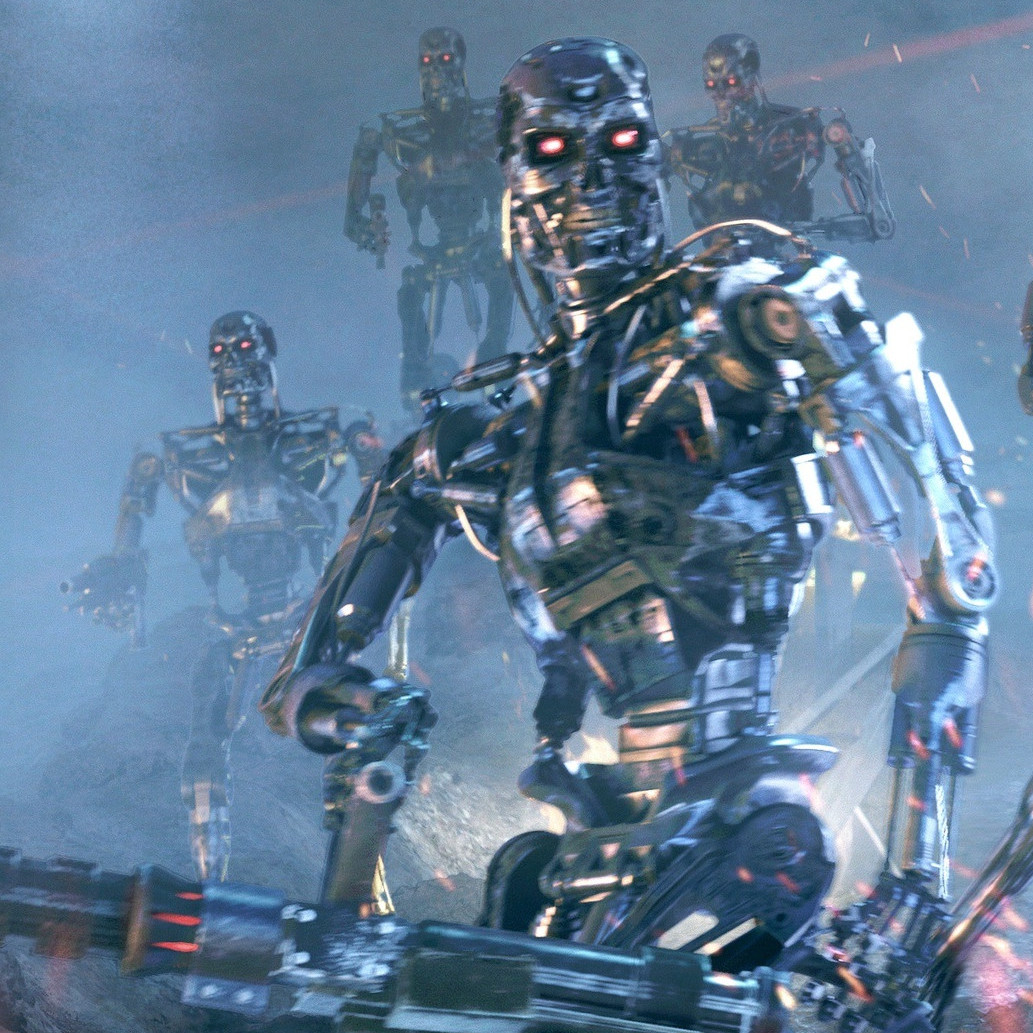
\includegraphics[width=\linewidth]{images/skynet.jpg}
        \caption{Surpass human performance in many tasks}
    \end{subfigure}
    \hspace{2em}
    \begin{subfigure}[t]{0.30\linewidth}
        \centering
        \captionsetup{justification=centering}
        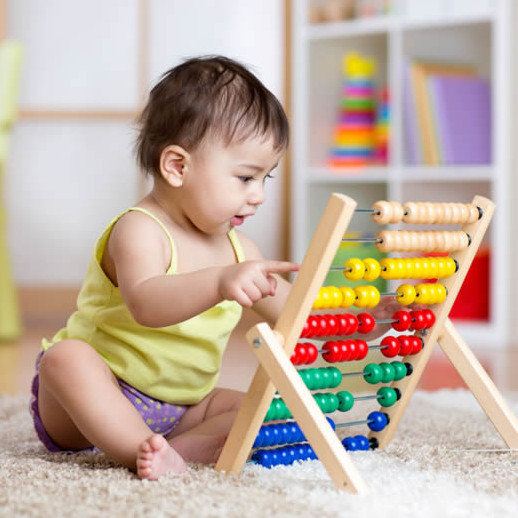
\includegraphics[width=\linewidth]{images/baby.jpg}
        \caption{Vulnerable against unknown threats}
    \end{subfigure}
\end{figure}
\end{frame}

%---------------------------------------------------------
\begin{frame}{Understanding the 4 key questions of Adversarial Attacks}
In the background study, I reviewed 4 key questions of adversarial attacks:
\begin{itemize}
    \item \textbf{What} is an adversarial example?
    \item \textbf{Why} is the ML model vulnerable to attack?
    \item \textbf{When} is the ML model vulnerable to attack?
    \item \textbf{How} to attack an ML model?
    % \item Why do adversarial examples transfer between models?
\end{itemize}

\end{frame}

%---------------------------------------------------------
\begin{frame}{What is an Adversarial Example?}
\begin{itemize}
    \item By adding a small perturbation to the existing input, the attacker can force the ML model to produce incorrect predictions.
    \item Adversarial perturbation/noise is not random.
\end{itemize}

\begin{examples}
    Applying Carlini \& Wagner $l_2$ attack on a deep neural network (DNN) model trained on MNIST
    \begin{figure}
        \centering
        \scriptsize
        
\includegraphics[width=0.7\linewidth]{images/from9to7.png}
        \caption{Clean Input (\textbf{Left}) + Perturbation (\textbf{Middle}) = Adversarial Example (\textbf{Right})}
    \end{figure}
    A DNN model with 99.6\% accuracy on the test set recognises the left image as \textbf{7}.
\end{examples}
\end{frame}

%---------------------------------------------------------
\begin{frame}{Why is the ML model vulnerable to attack?}
\label{decision_boundary}

\begin{block}{Assumption of ML model}
Training data is representative of the test data.
\end{block}

In the simplest way, adversarial examples move the clean examples to somewhere near the decision boundary

\begin{figure}
    \centering
    \small
    \begin{subfigure}[t]{0.38\linewidth}
        \centering
        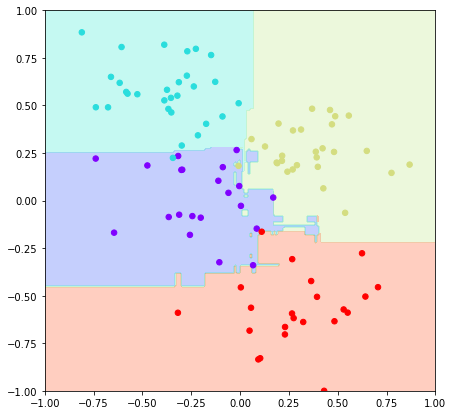
\includegraphics[width=\linewidth]{images/dt_test_set.png}
        \caption{Evaluating the test set on a Random Forest model}
    \end{subfigure}
    \hspace{2em}
    \begin{subfigure}[t]{0.38\linewidth}
        \centering
        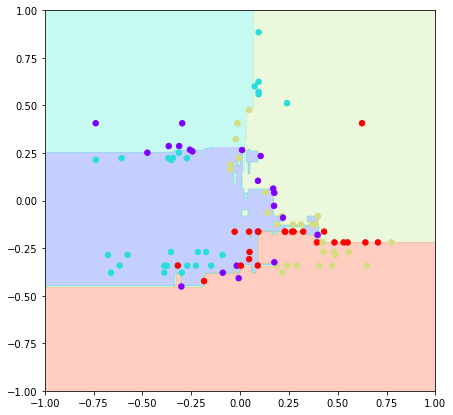
\includegraphics[width=\linewidth]{images/dt_adv_examples.png}
        \caption{Untargeted White-box Random Forest Attack}
    \end{subfigure}
    \caption{A Random Forest model on a 2D synthetic dataset}
\end{figure}

\hyperlink{reliability}{\beamerreturnbutton{Reliability Stage}}
\hyperlink{ad}{\beamerreturnbutton{Applicability Domain}}
\end{frame}

%---------------------------------------------------------
\begin{frame}{What is the goal of the adversary?}
\begin{itemize}
    \item Confidence reduction (\textit{Does not affect accuracy})
    \item Untargeted misclassification (\textit{High success rate}: Any label other than the correct one is acceptable)
    \item Targeted misclassification (Looking for a specific label)
    \item Source/target misclassification (\textit{Lowest success rate}: Given the input and the label)
\end{itemize}

\begin{block}{Successful Attack}
An adversarial example achieves its goal before it exhausts the searching space within the upper bound.
\end{block}

No difference between targeted and untargeted in binary classification (e.g. Spam filter)
\end{frame}

%---------------------------------------------------------
\begin{frame}{Definition of Success}
\begin{alertblock}{What is NOT Adversarial Attack?}
If the maximum perturbation is undefined, you can simple replace the current input with a completely different one, and call it a success attack. 
\end{alertblock}

\begin{block}{Successful Attack}
An adversarial example achieves its goal before it exhausts the searching space within the \textbf{upper bound}.
\end{block}

There are different interpretations of the maximum \textbf{upper bound}.

\begin{itemize}
    \item \textbf{$l_\infty$}: The largest change among all features (e.g. [1, -6, 2], [2, 0, 3], $l_\infty = 6$)
    \item \textbf{$l_2$}: The Euclidean distance 
    \item \textbf{$l_0$}: Counting the number of changes (e.g. [1, -6, 2], [1, 0, 2], $l_0 = 1$)
\end{itemize}
\end{frame}

%---------------------------------------------------------
\begin{frame}{When is the ML model vulnerable to attack?}
\begin{itemize}
    \item \textbf{Poisoning Attacks}: Injecting a small fraction of poisoning samples during the \textbf{training}
    \item \textbf{Evasion Attacks}: Manipulate a single data point to force the model to make a false negative (type II) error at \textbf{runtime}
\end{itemize}

\begin{figure}
    \centering
    \small
    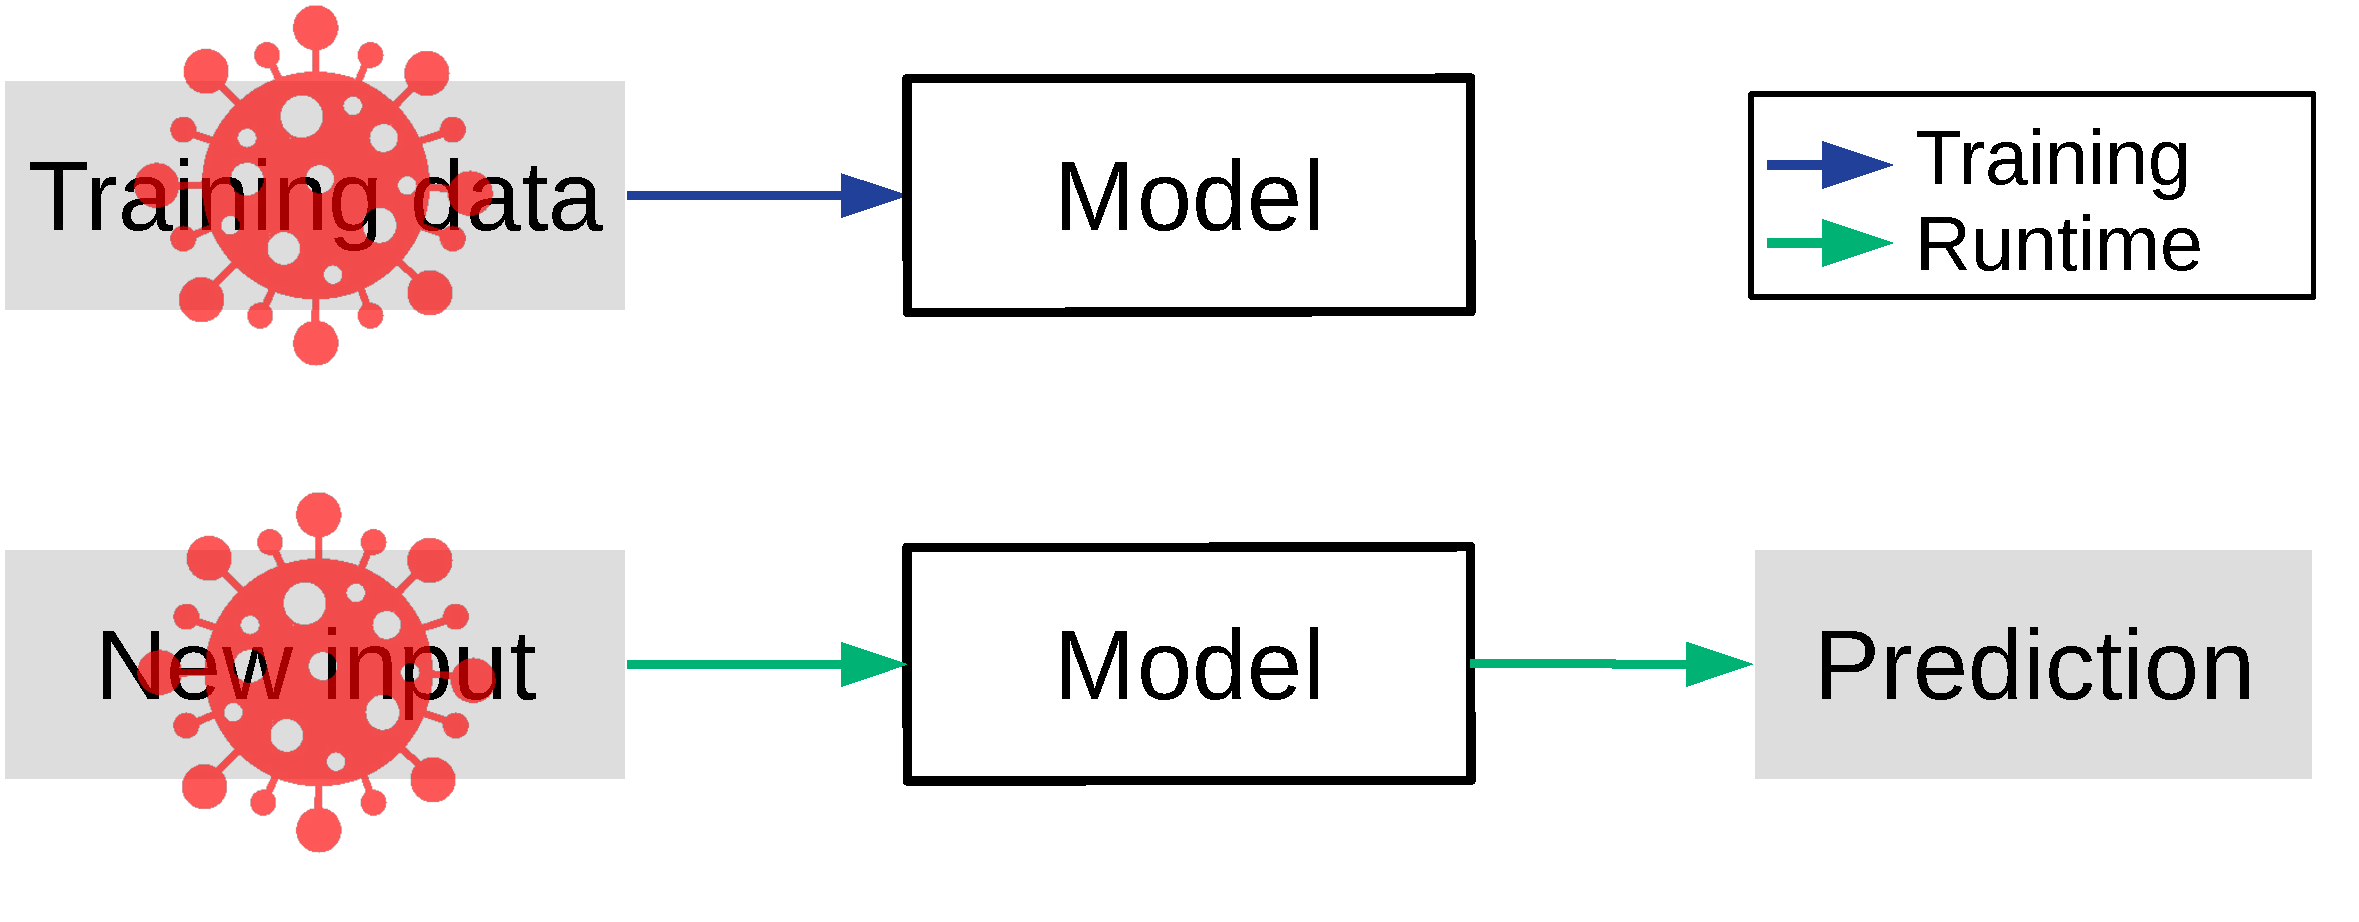
\includegraphics[width=0.8\linewidth]{images/attack_models.pdf}
    \caption{Poisoning Attack (Top) and Evasion Attack (Bottom)}
    \label{fig:surrogate}
\end{figure}

In my \nth{1} year, I'm focusing on defending evasion attacks. \\
I will explore poisoning attacks in the next stage.

\end{frame}

%---------------------------------------------------------
\begin{frame}{Threat models for Evasion Attacks}
The threat Model is used to determine the difficulty of an evasion attack.

\begin{block}{Prior}
Adversaries always have a basic understanding of the data structure.
\end{block}

Based on the adversary's knowledge

\begin{itemize}
    \item Zero-knowledge: black-box with probing\footnote{The universal adversarial examples (black-box without probing) do exist.} (\textit{Low success rate})
    \item Limited-knowledge: grey-box (\textit{Most common})
    \item Perfect-knowledge: white-box (\textit{High success rate})
\end{itemize}

\begin{alertblock}{Evasion Attack Assumption}
Both data and model are read-only, the adversaries do not alter the model.\\
No poisoning examples in the training data.
\end{alertblock}
\end{frame}

%---------------------------------------------------------
\begin{frame}{How to attack an ML model?}
\begin{block}{Basic Concept of Attacking a Neural Network (NN) model}
Training minimises the \textbf{loss function}. Adversarial examples \textbf{maximise} the \textbf{loss function} by reversing the gradient in the backpropagation.
\end{block}

{
\small
The attacks I have studied:
\textbf{White-box Attacks:}
\begin{itemize}
    \item \textbf{Fast Gradient Sign Method} (FGSM) for $l_\infty$ untargeted attack 
    \item \textbf{Basic Iterative Method} (BIM) for $l_\infty$ targeted attack 
    \item \textbf{Carlini and Wagner} $l_2$ (C\&W) targeted attack 
    \item \textbf{DeepFool} for $l_2$ (C\&W) untargeted attack 
    \item \textbf{Jacobian based Saliency Map Approach} (JSMA) for $l_0$ targeted attack 
    \item \textbf{Decision Tree Attack} for attacking Decision Tree models
\end{itemize}

Implemented a GPU version of the C\&W $l_2$ attack using \textit{PyTorch}

\textbf{Black-box Attacks:}
\begin{itemize}
    \item Training \textbf{surrogate models}
    \item \textbf{Zeroth Order Optimisation} (ZOO) attack
    \item \textbf{Boundary Attack} for attacking SVM
\end{itemize}
}

\end{frame}

%---------------------------------------------------------
\begin{frame}{Adversarial Examples}
\label{adv_examples}

\begin{figure}
    \centering
    \tiny
    \begin{subfigure}[t]{0.23\linewidth}
        \centering
        \captionsetup{justification=centering}
        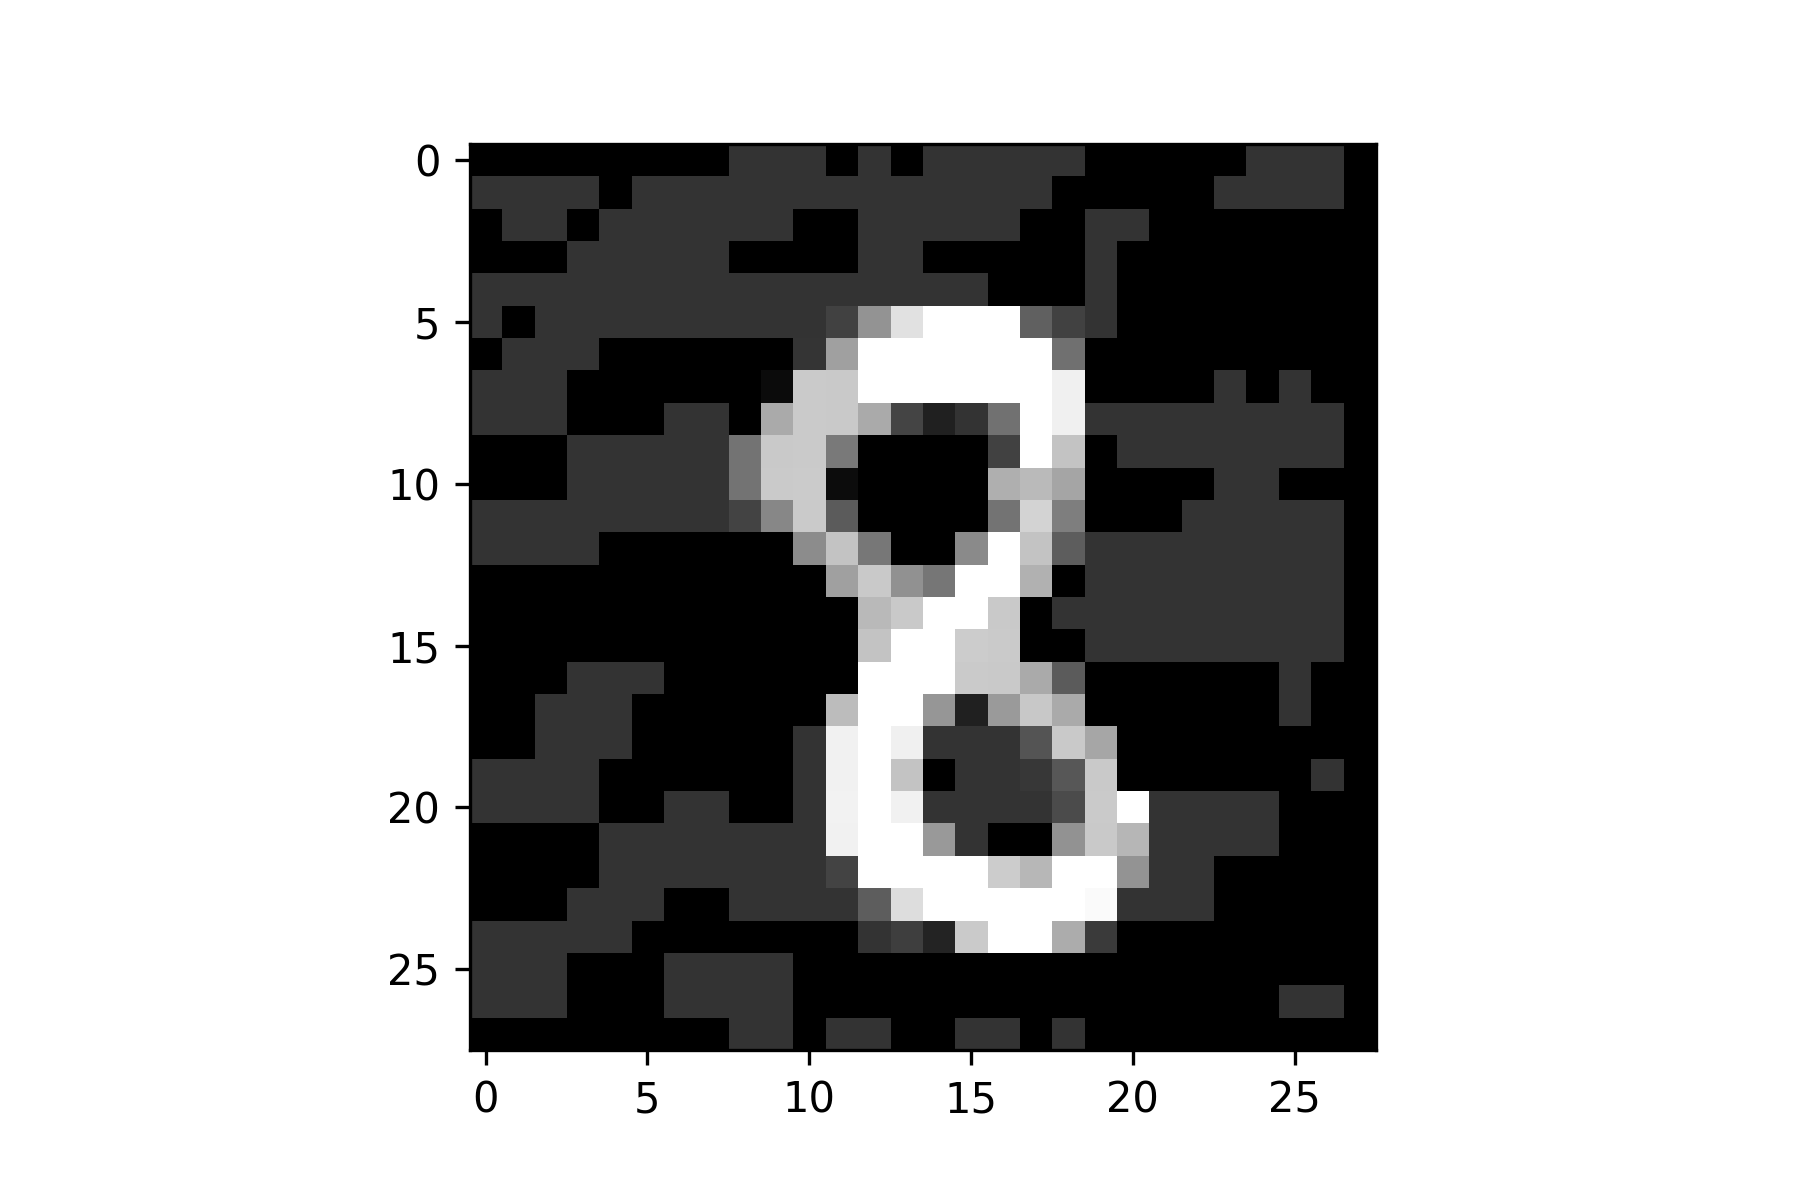
\includegraphics[width=\linewidth]{images/FGSM_2.png}
        \caption{FGSM\\Prediction: 2}
    \end{subfigure}
    \begin{subfigure}[t]{0.23\linewidth}
        \centering
        \captionsetup{justification=centering}
        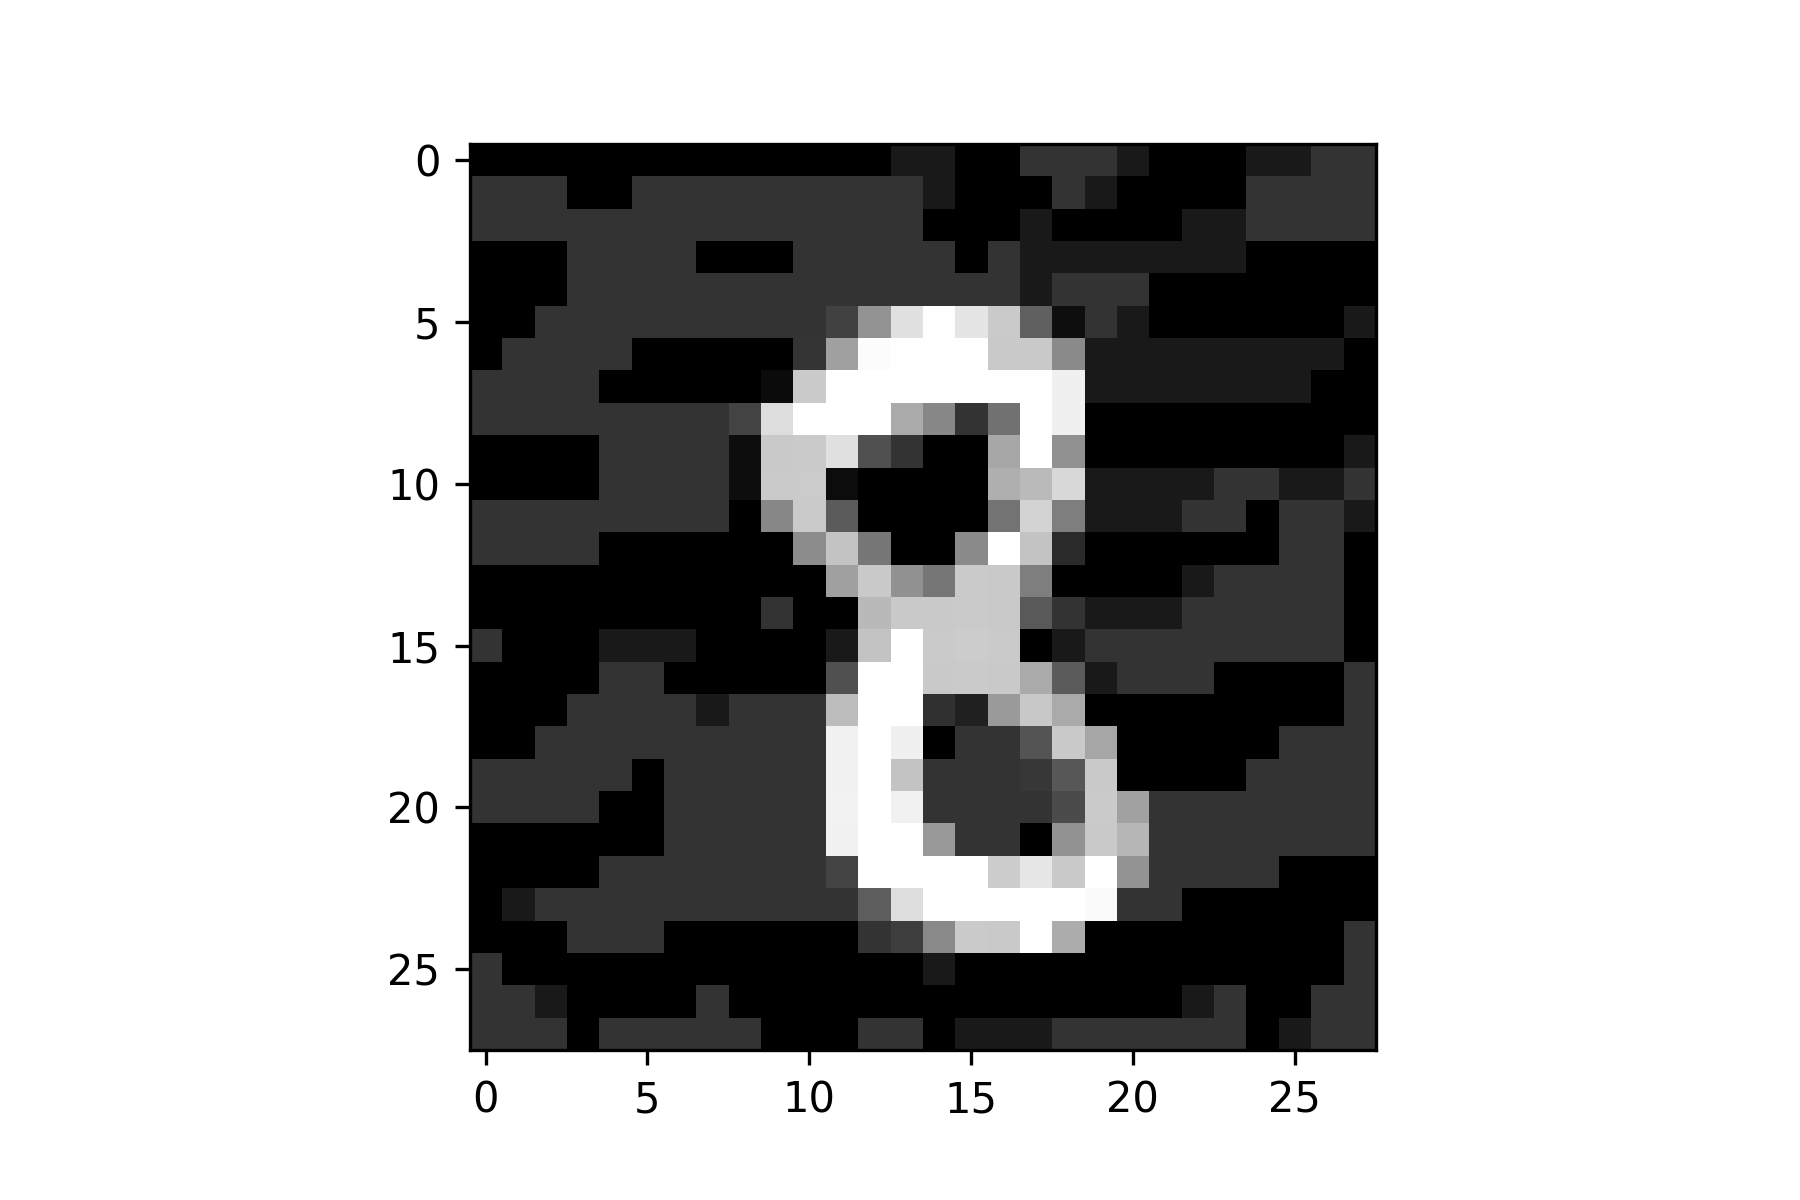
\includegraphics[width=\linewidth]{images/BIM_2.png}
        \caption{BIM\\Prediction: 2}
    \end{subfigure}
    \begin{subfigure}[t]{0.23\linewidth}
        \centering
        \captionsetup{justification=centering}
        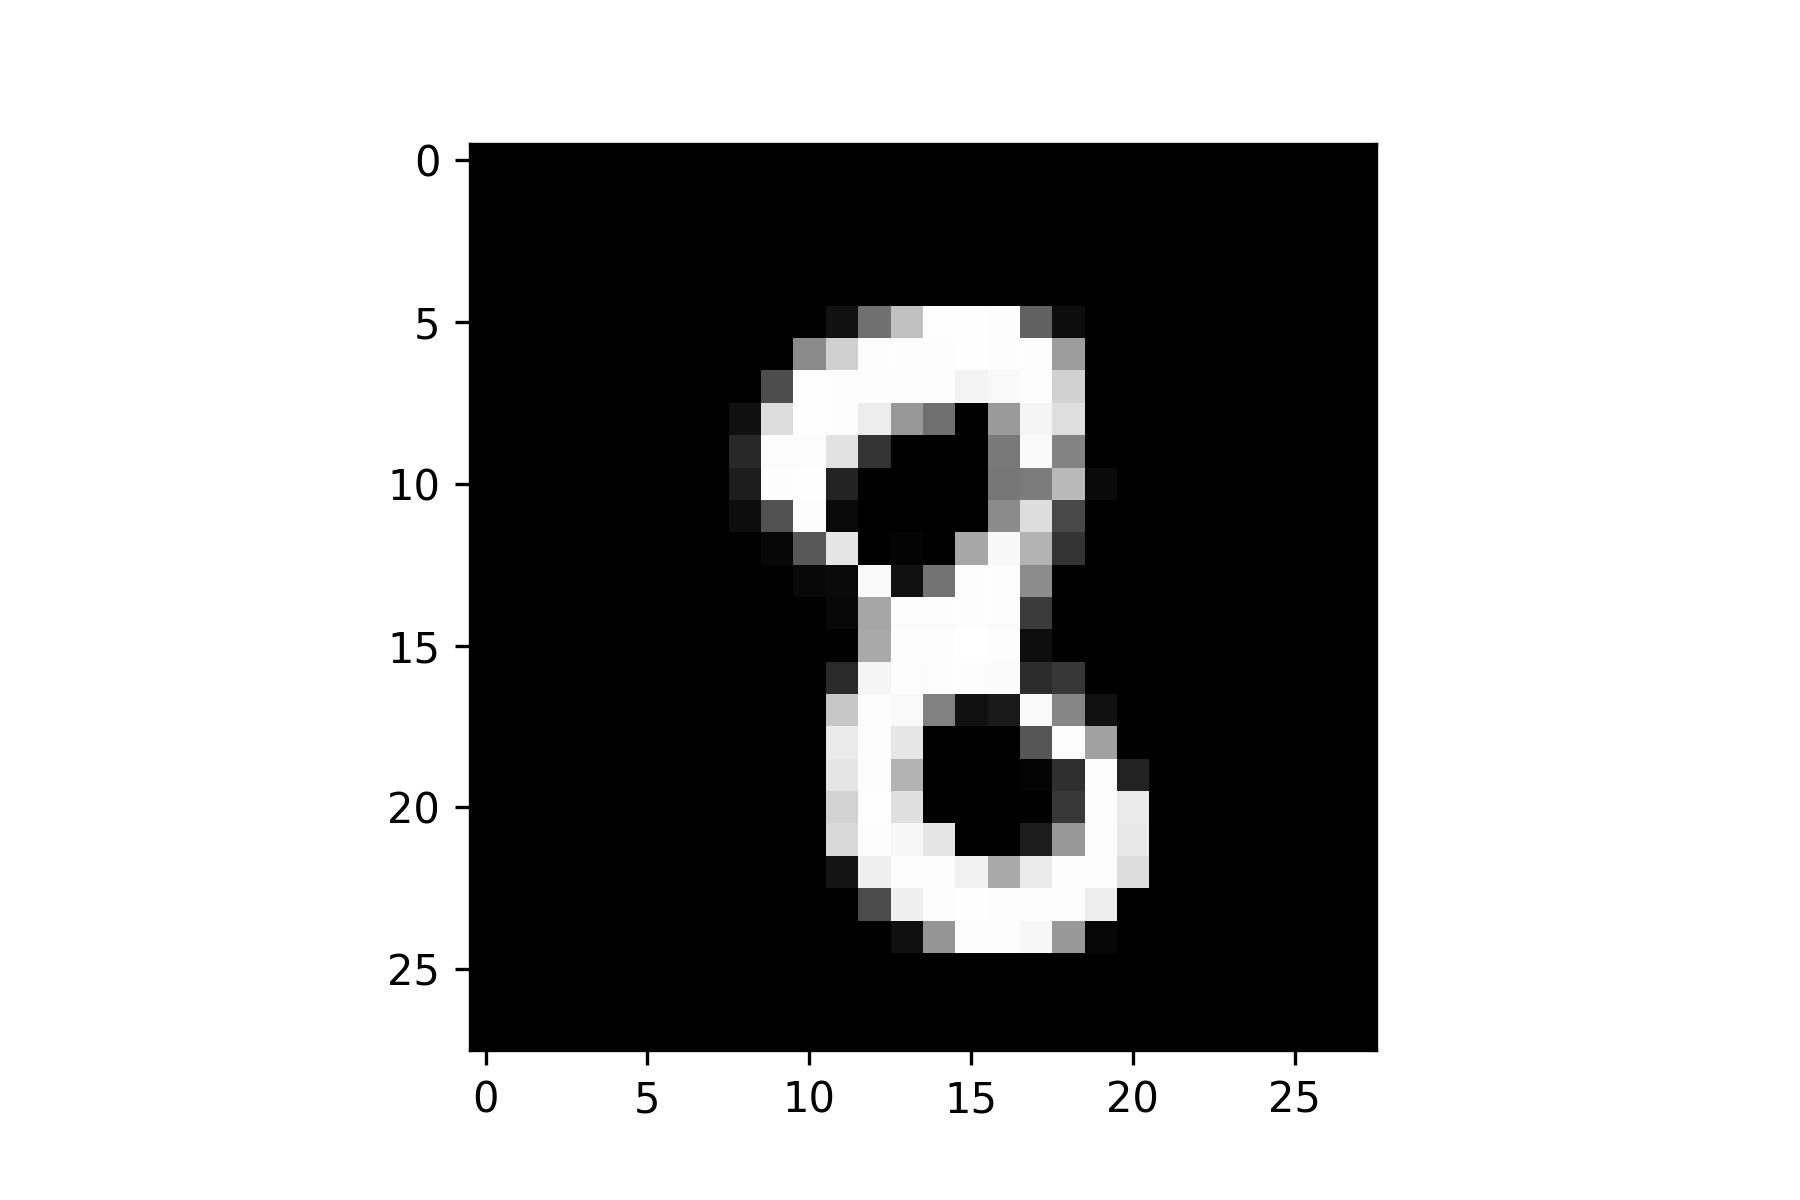
\includegraphics[width=\linewidth]{images/CW_2.png}
        \caption{C\&W\\Prediction: 2}
    \end{subfigure}
    \begin{subfigure}[t]{0.23\linewidth}
        \centering
        \captionsetup{justification=centering}
        \captionsetup{justification=centering}
        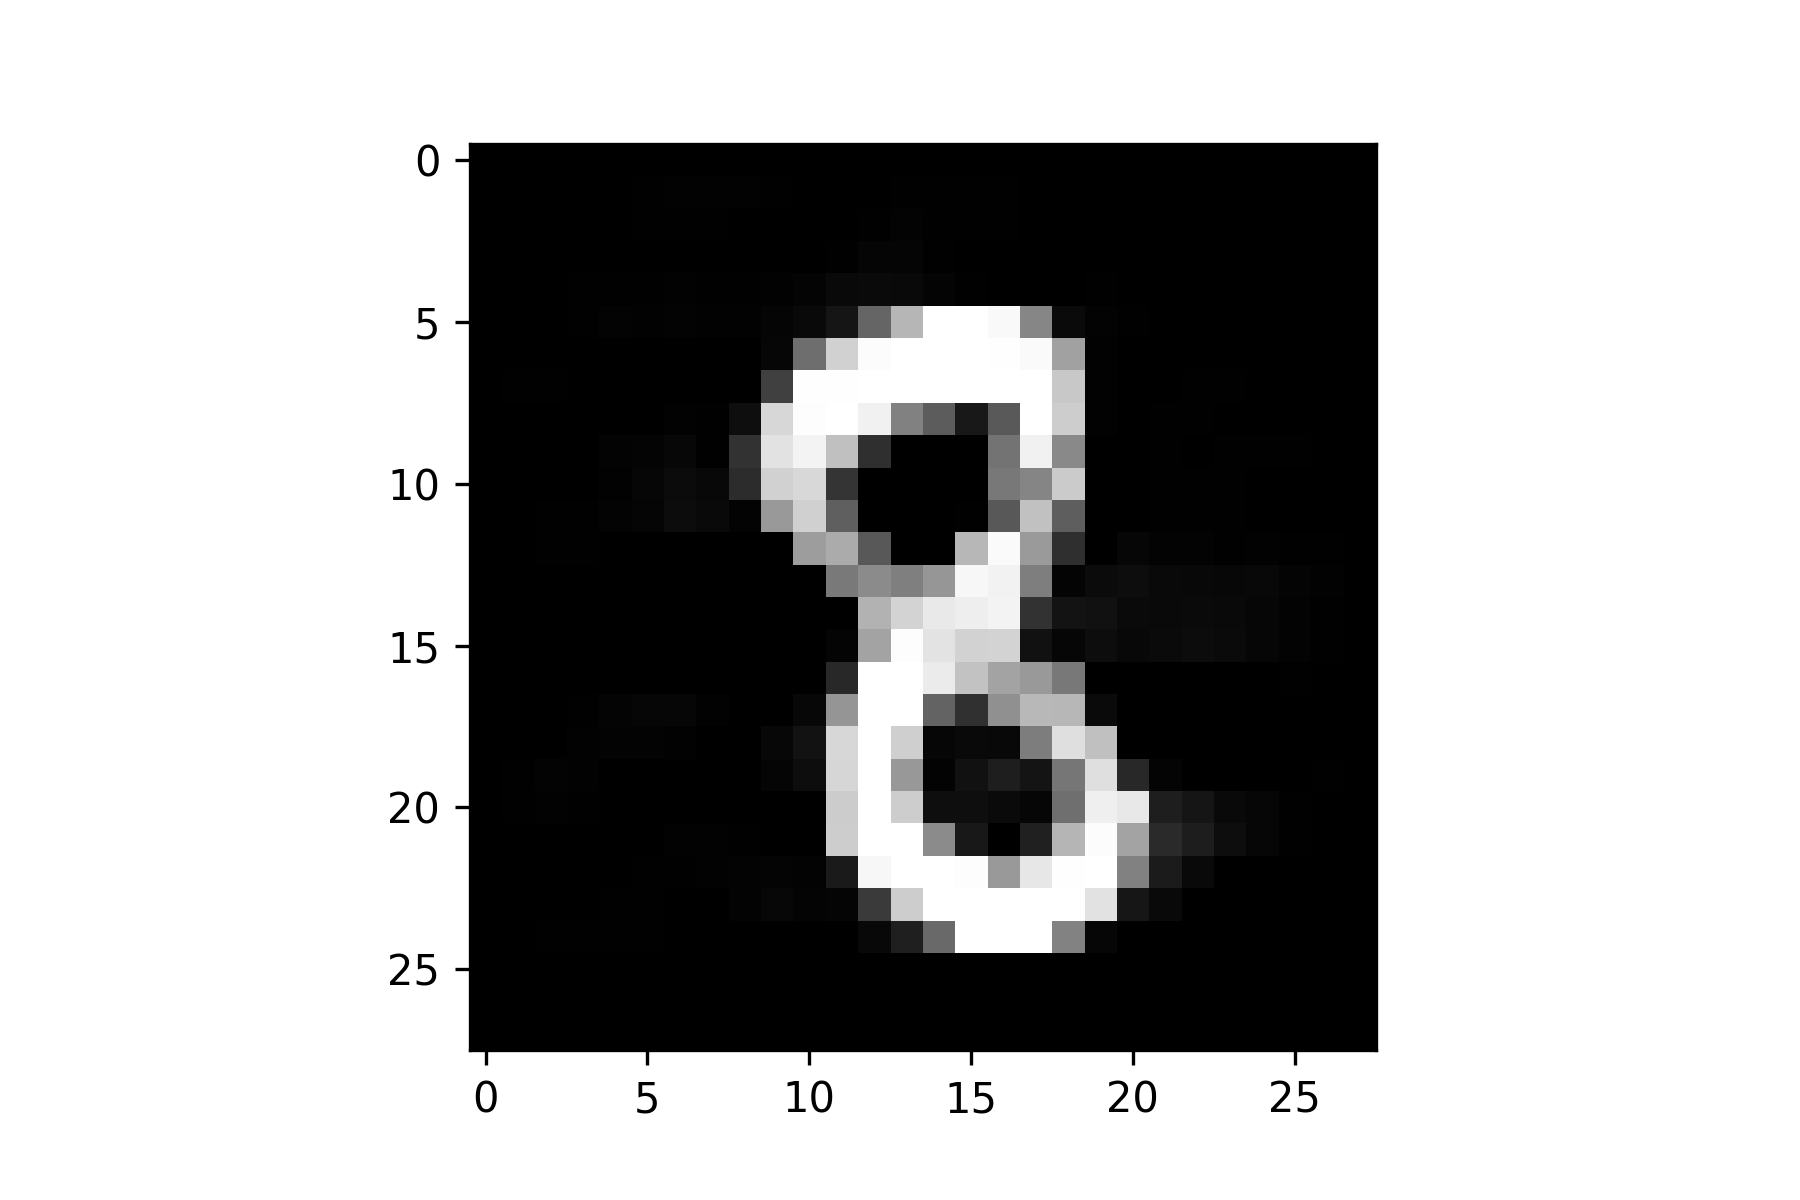
\includegraphics[width=\linewidth]{images/DeepFool_2.png}
        \caption{DeepFool\\Prediction: 2}
    \end{subfigure}
    \begin{subfigure}[t]{0.23\linewidth}
        \centering
        \captionsetup{justification=centering}
        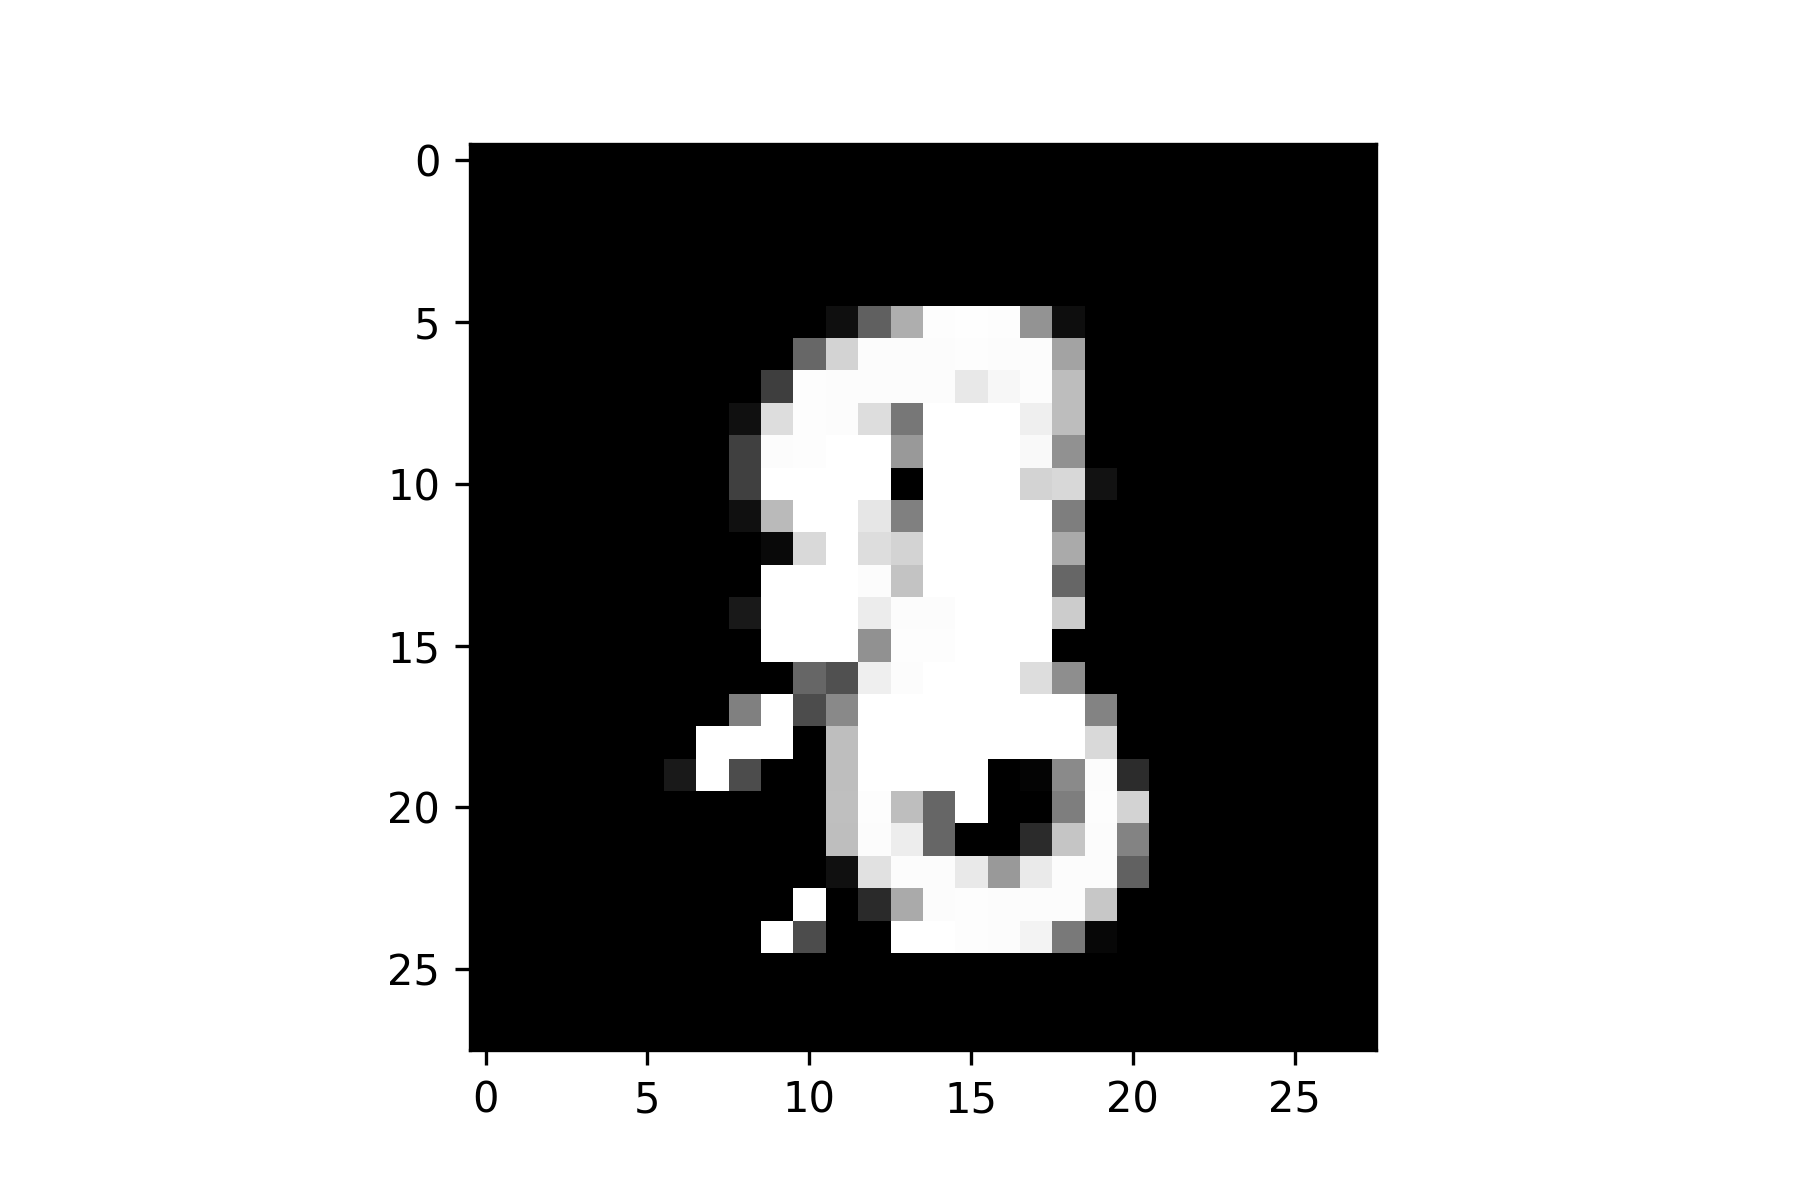
\includegraphics[width=\linewidth]{images/JSMA_4.png}
        \caption{JSMA\\Prediction: 4}
    \end{subfigure}
    \begin{subfigure}[t]{0.23\linewidth}
        \centering
        \captionsetup{justification=centering}
        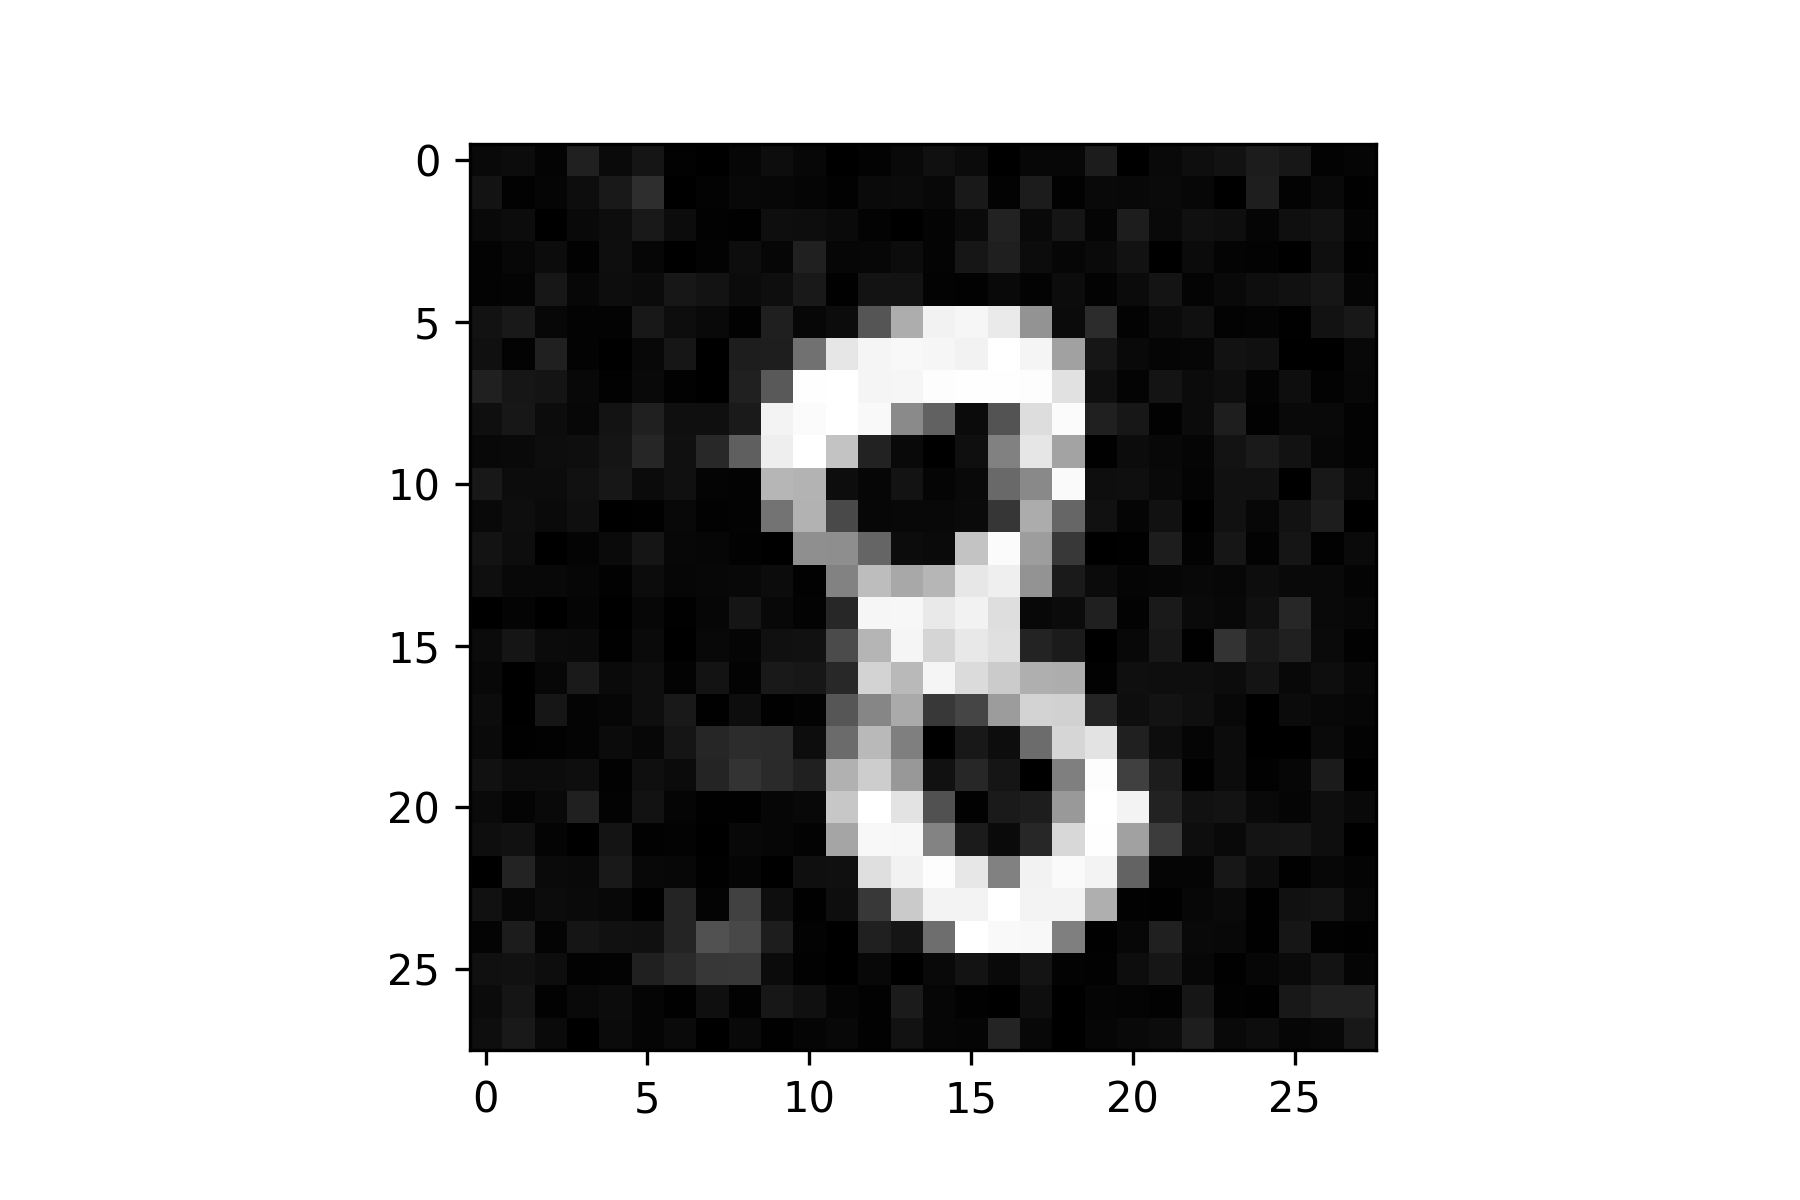
\includegraphics[width=\linewidth]{images/BoundaryAttack_3.png}
        \caption{Boundary Attack\\Prediction: 2}
    \end{subfigure}
    \begin{subfigure}[t]{0.23\linewidth}
        \centering
        \captionsetup{justification=centering}
        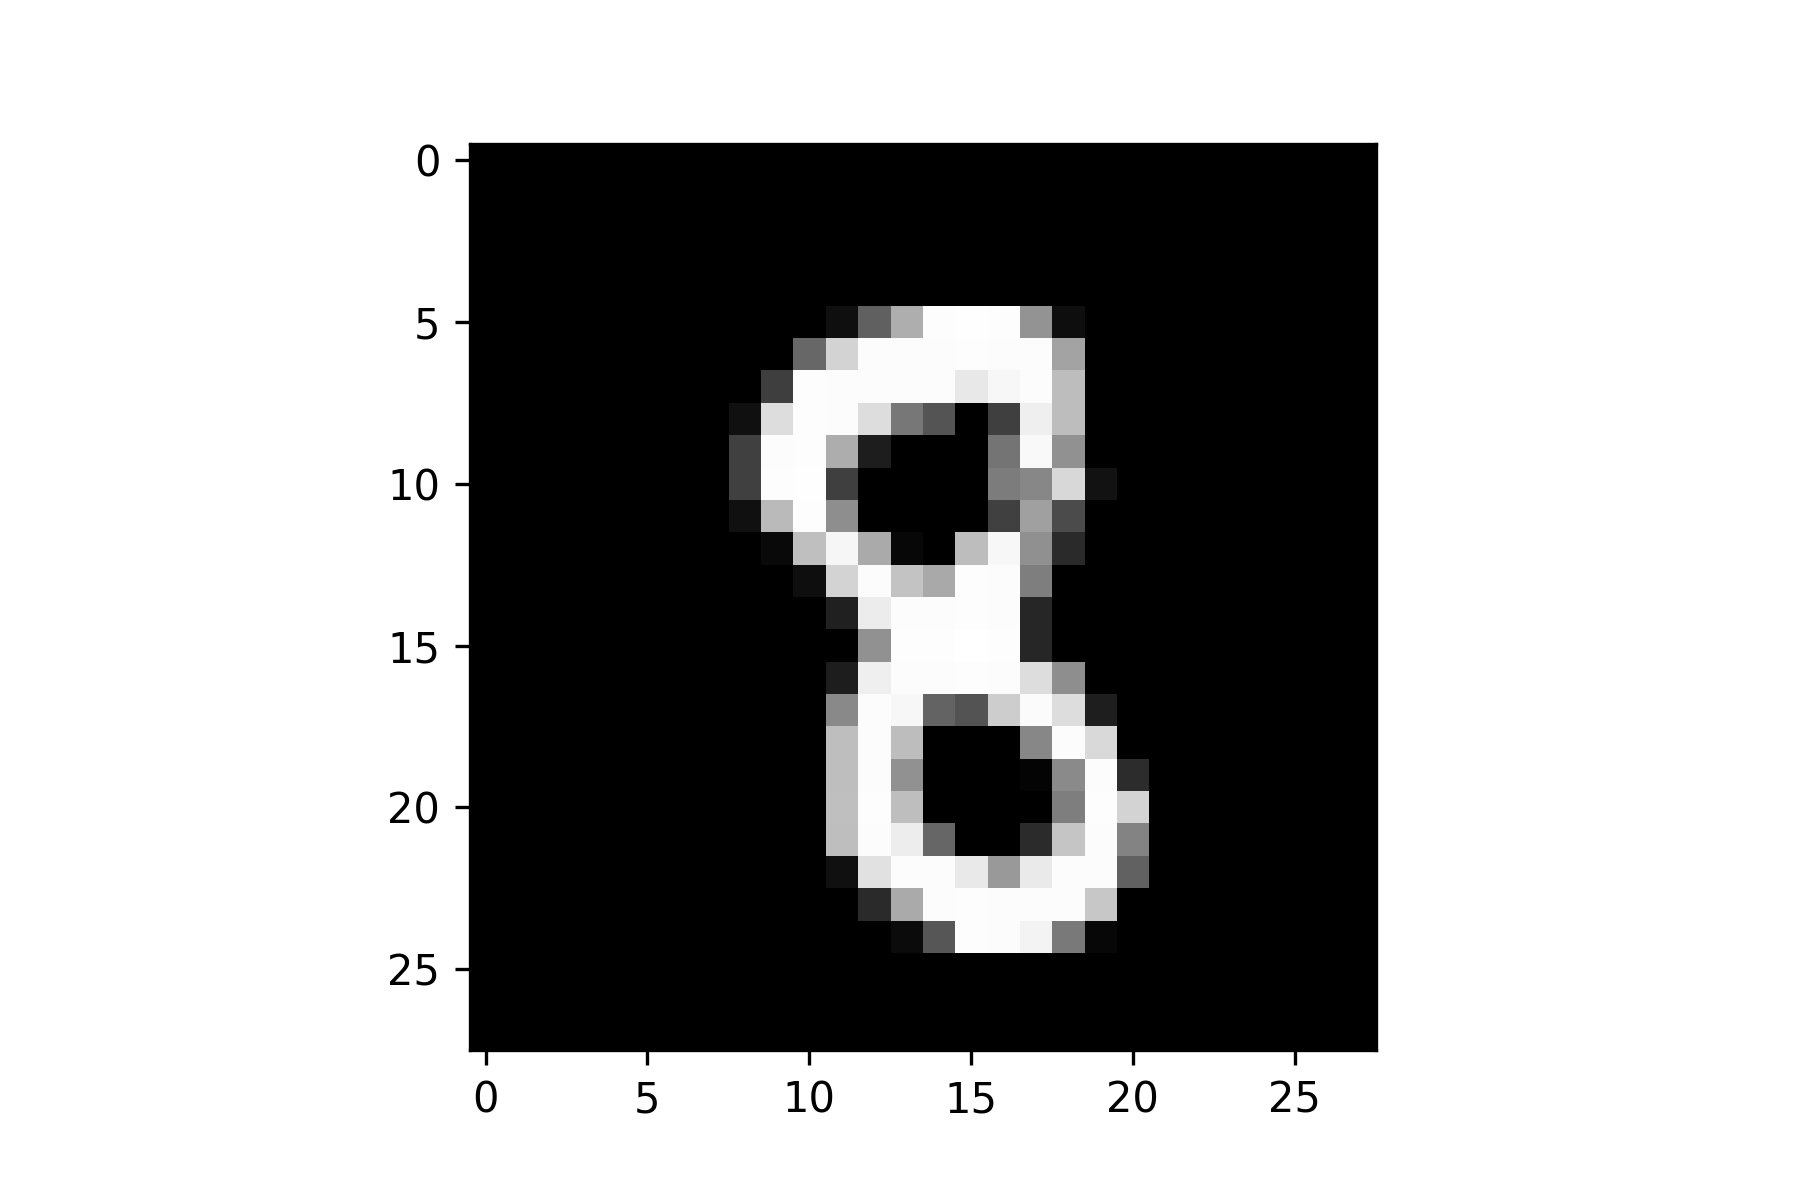
\includegraphics[width=\linewidth]{images/Zoo_8.png}
        \caption{Zoo\\Failed}
    \end{subfigure}
    \begin{subfigure}[t]{0.23\linewidth}
        \centering
        \captionsetup{justification=centering}
        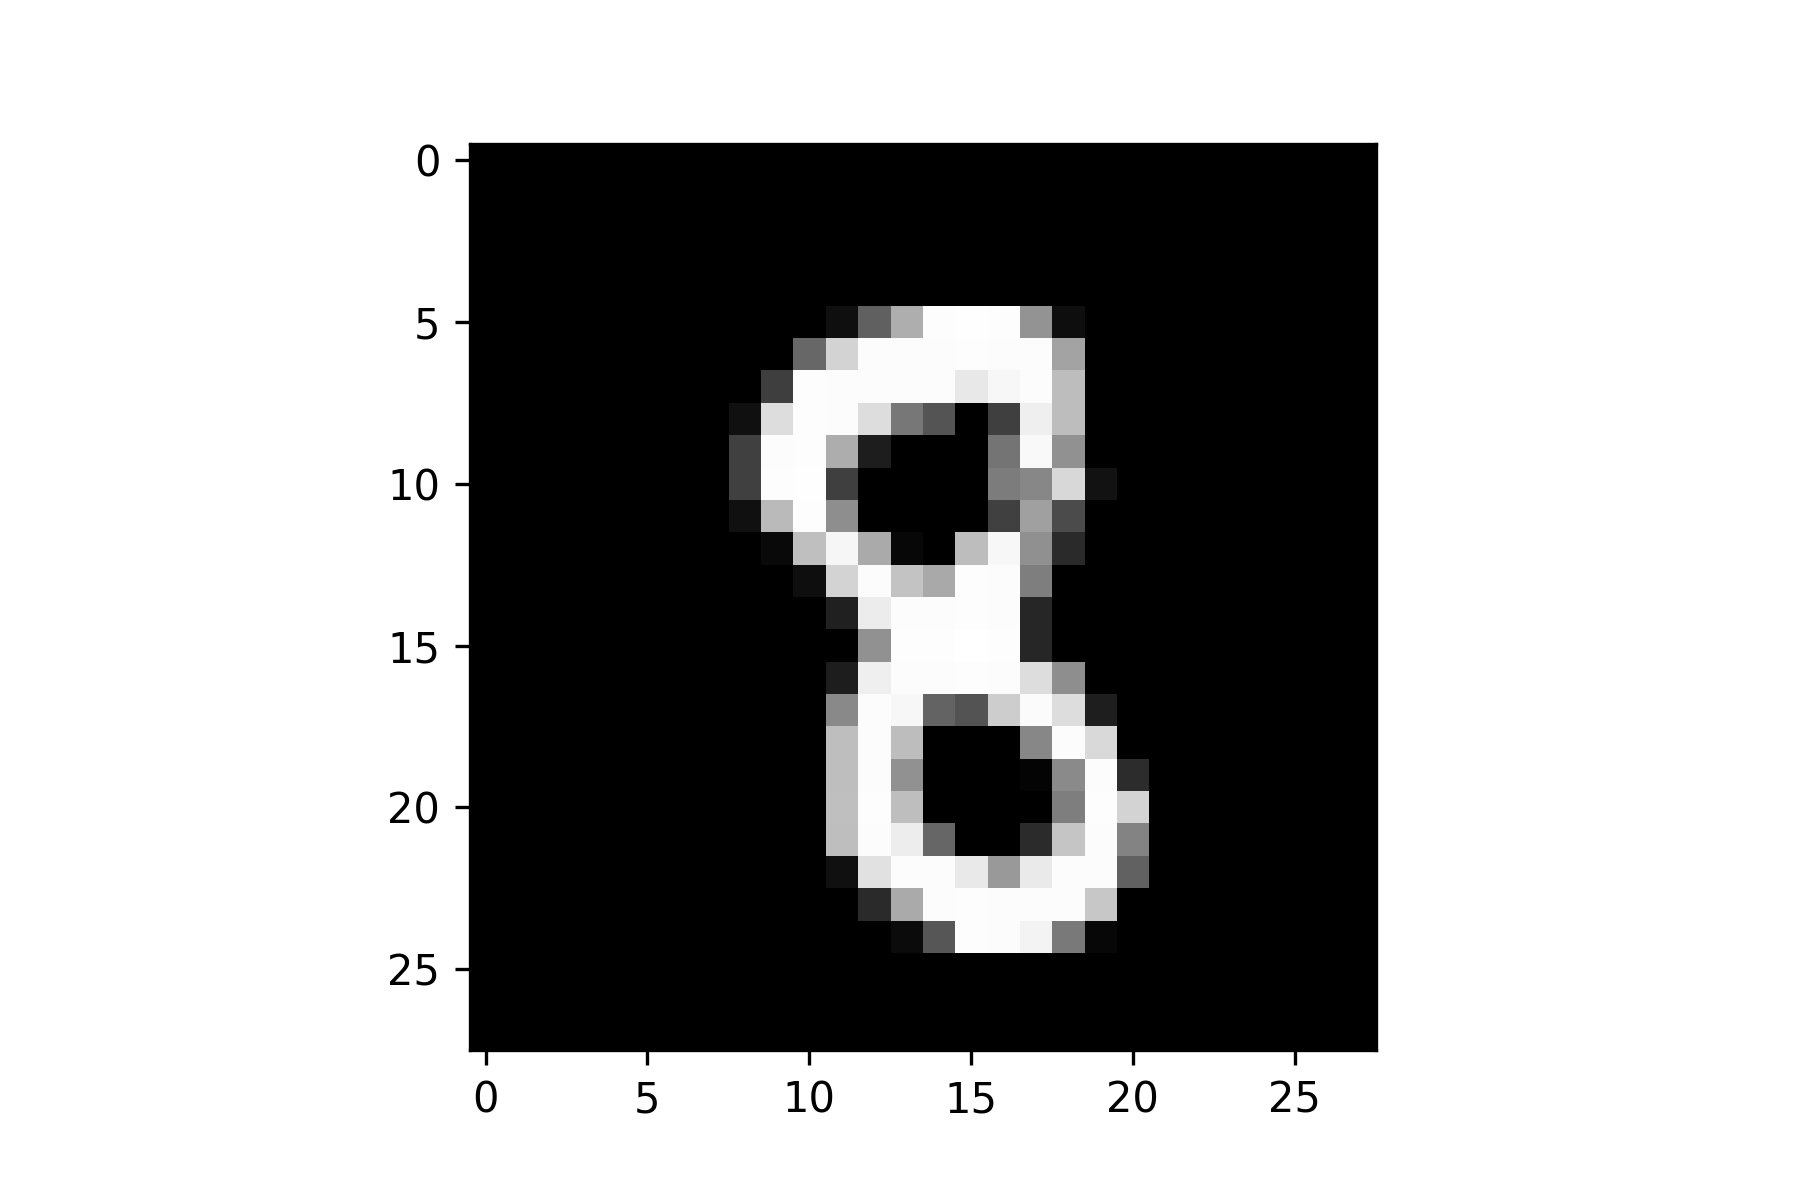
\includegraphics[width=\linewidth]{images/PixelAttack_8.png}
        \caption{Pixel Attack\\Failed}
    \end{subfigure}
    \begin{subfigure}[t]{0.23\linewidth}
        \centering
        \captionsetup{justification=centering}
        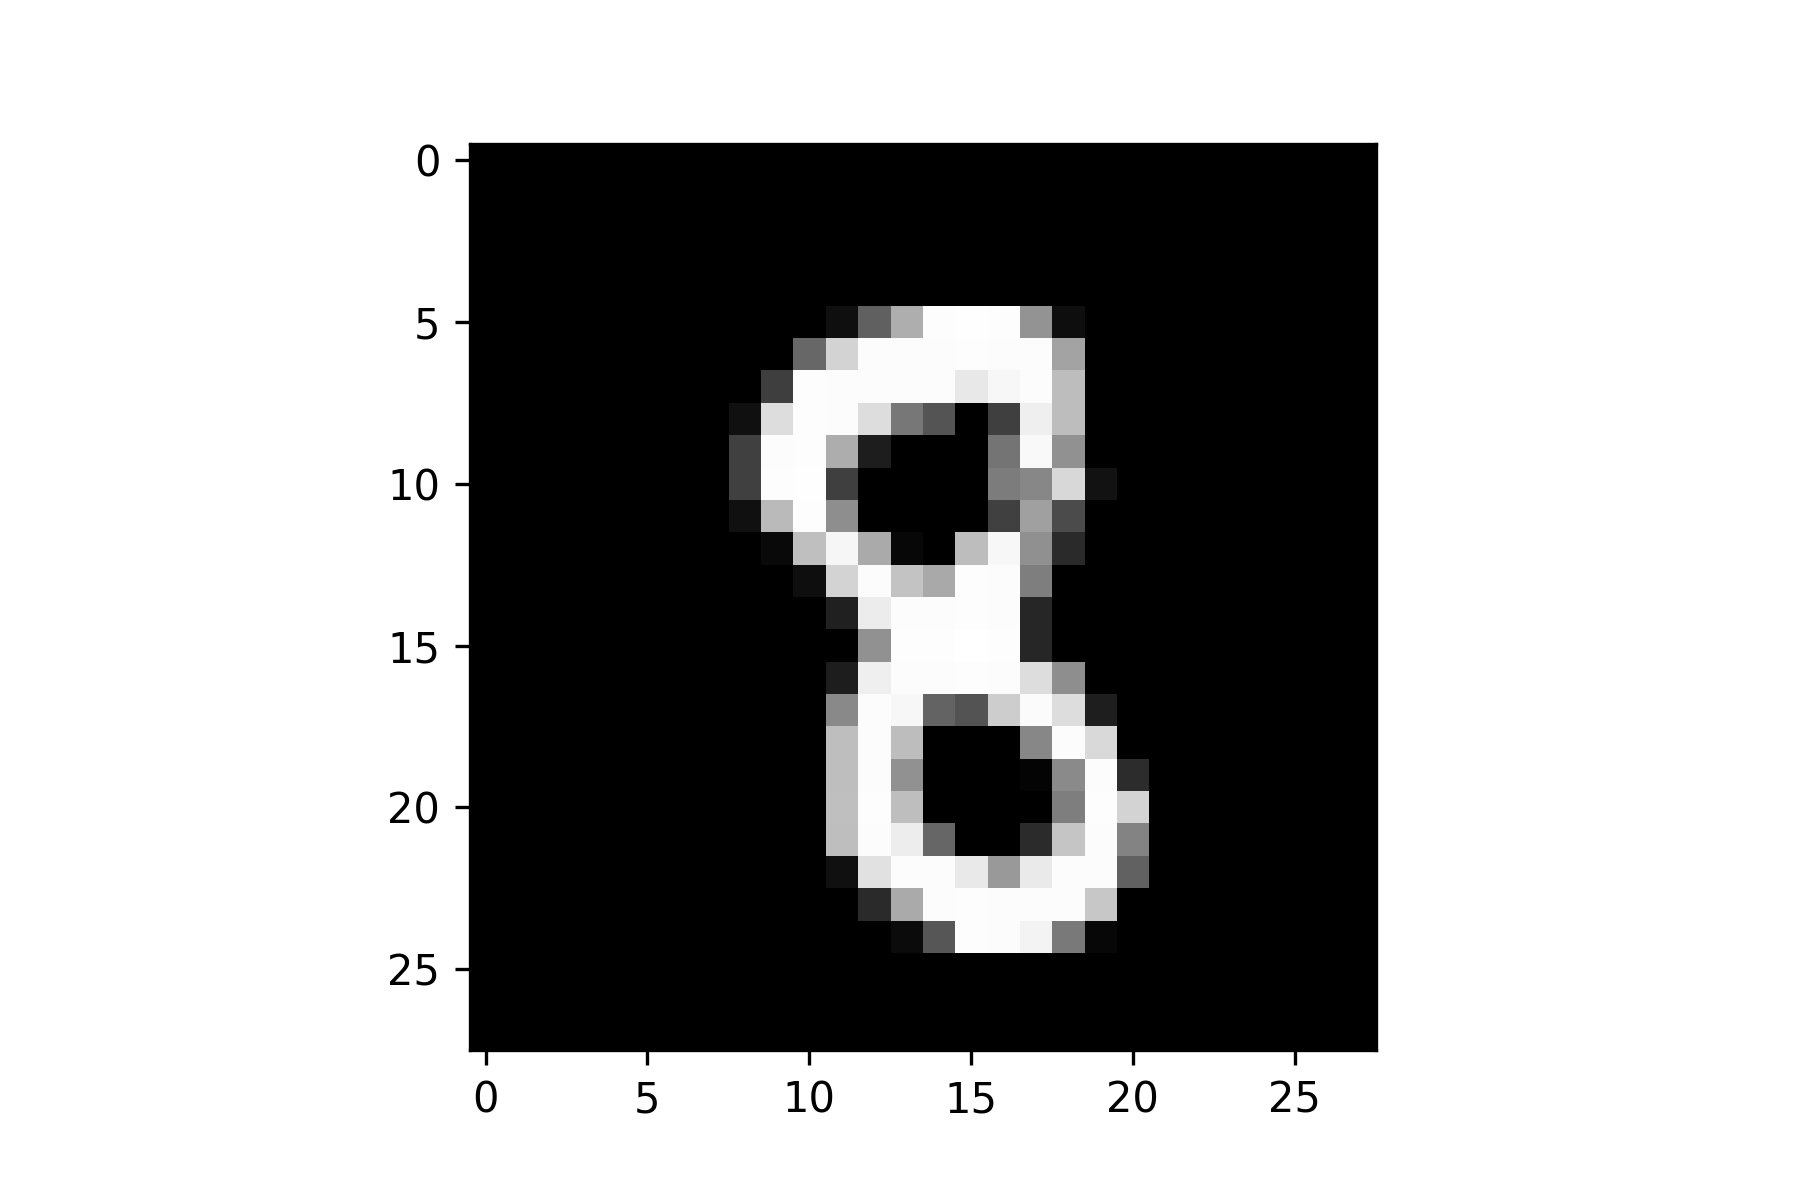
\includegraphics[width=\linewidth]{images/clean_8.png}
        \caption{Clean input\\Prediction: 8}
        \label{fig:clean}
    \end{subfigure}
\end{figure}

\hyperlink{preprocessing}{\beamerreturnbutton{Preprocessing}}
\hyperlink{adv_training}{\beamerreturnbutton{Adversarial Retraining}}
\hyperlink{stats}{\beamerreturnbutton{Statistical Analysis}}
\end{frame}

%---------------------------------------------------------
\begin{frame}{Accuracy of models under adversarial attacks}
\begin{table}
    \centering
    \footnotesize
    \begin{tabular}{|l|c|c|c|c|c|c|}
        \hline
        {Dataset} & {Clean(\%)} & {FGSM(\%)} & {BIM(\%)} & {DeepFool(\%)} & {C\&W(\%)} & {JSMA(\%)} \\
        \hline
        MNIST & 99.60 & 70.50 & 0.00 & 36.60 & 10.30 & 0.00 \\
        CIFAR-Basic & 83.60 & 2.30 & 0.00 & 42.10 & 9.10 & 0.00 \\
        CIFAR-ResNet & 82.90 & 7.80 & 0.00 & 20.20 & 12.00 & 0.00 \\
        SVHN-Basic & 92.20 & 4.50 & 0.00 & 34.00 & 11.70 & 0.00 \\
        SVHN-ResNet & 90.00 & 7.70 & 0.00 & 19.00 & 9.80 & 0.10 \\
        Iris & 93.33 & 25.00 & 0.00 & 13.33 & 20.00 & \\
        BankNote & 100.00 & 0.73 & 0.00 & 15.69 & 45.62 & \\
        WheatSeed & 90.48 & 23.81 & 07.14 & 4.76 & 21.43 & \\
        HTRU2 & 97.70 & 2.80 & 0.60 & 21.30 & 17.00 & \\
        BreastCancer & 97.37 & 2.63 & 0.88 & 07.89 & 52.63 & \\
        \hline
    \end{tabular}
    \caption{Model accuracy under the white-box evasion attacks}
    \label{table:adv_acc}
\end{table}
\end{frame}

%---------------------------------------------------------
\begin{frame}{Surrogate Models}
\begin{figure}
    \centering
    \small
    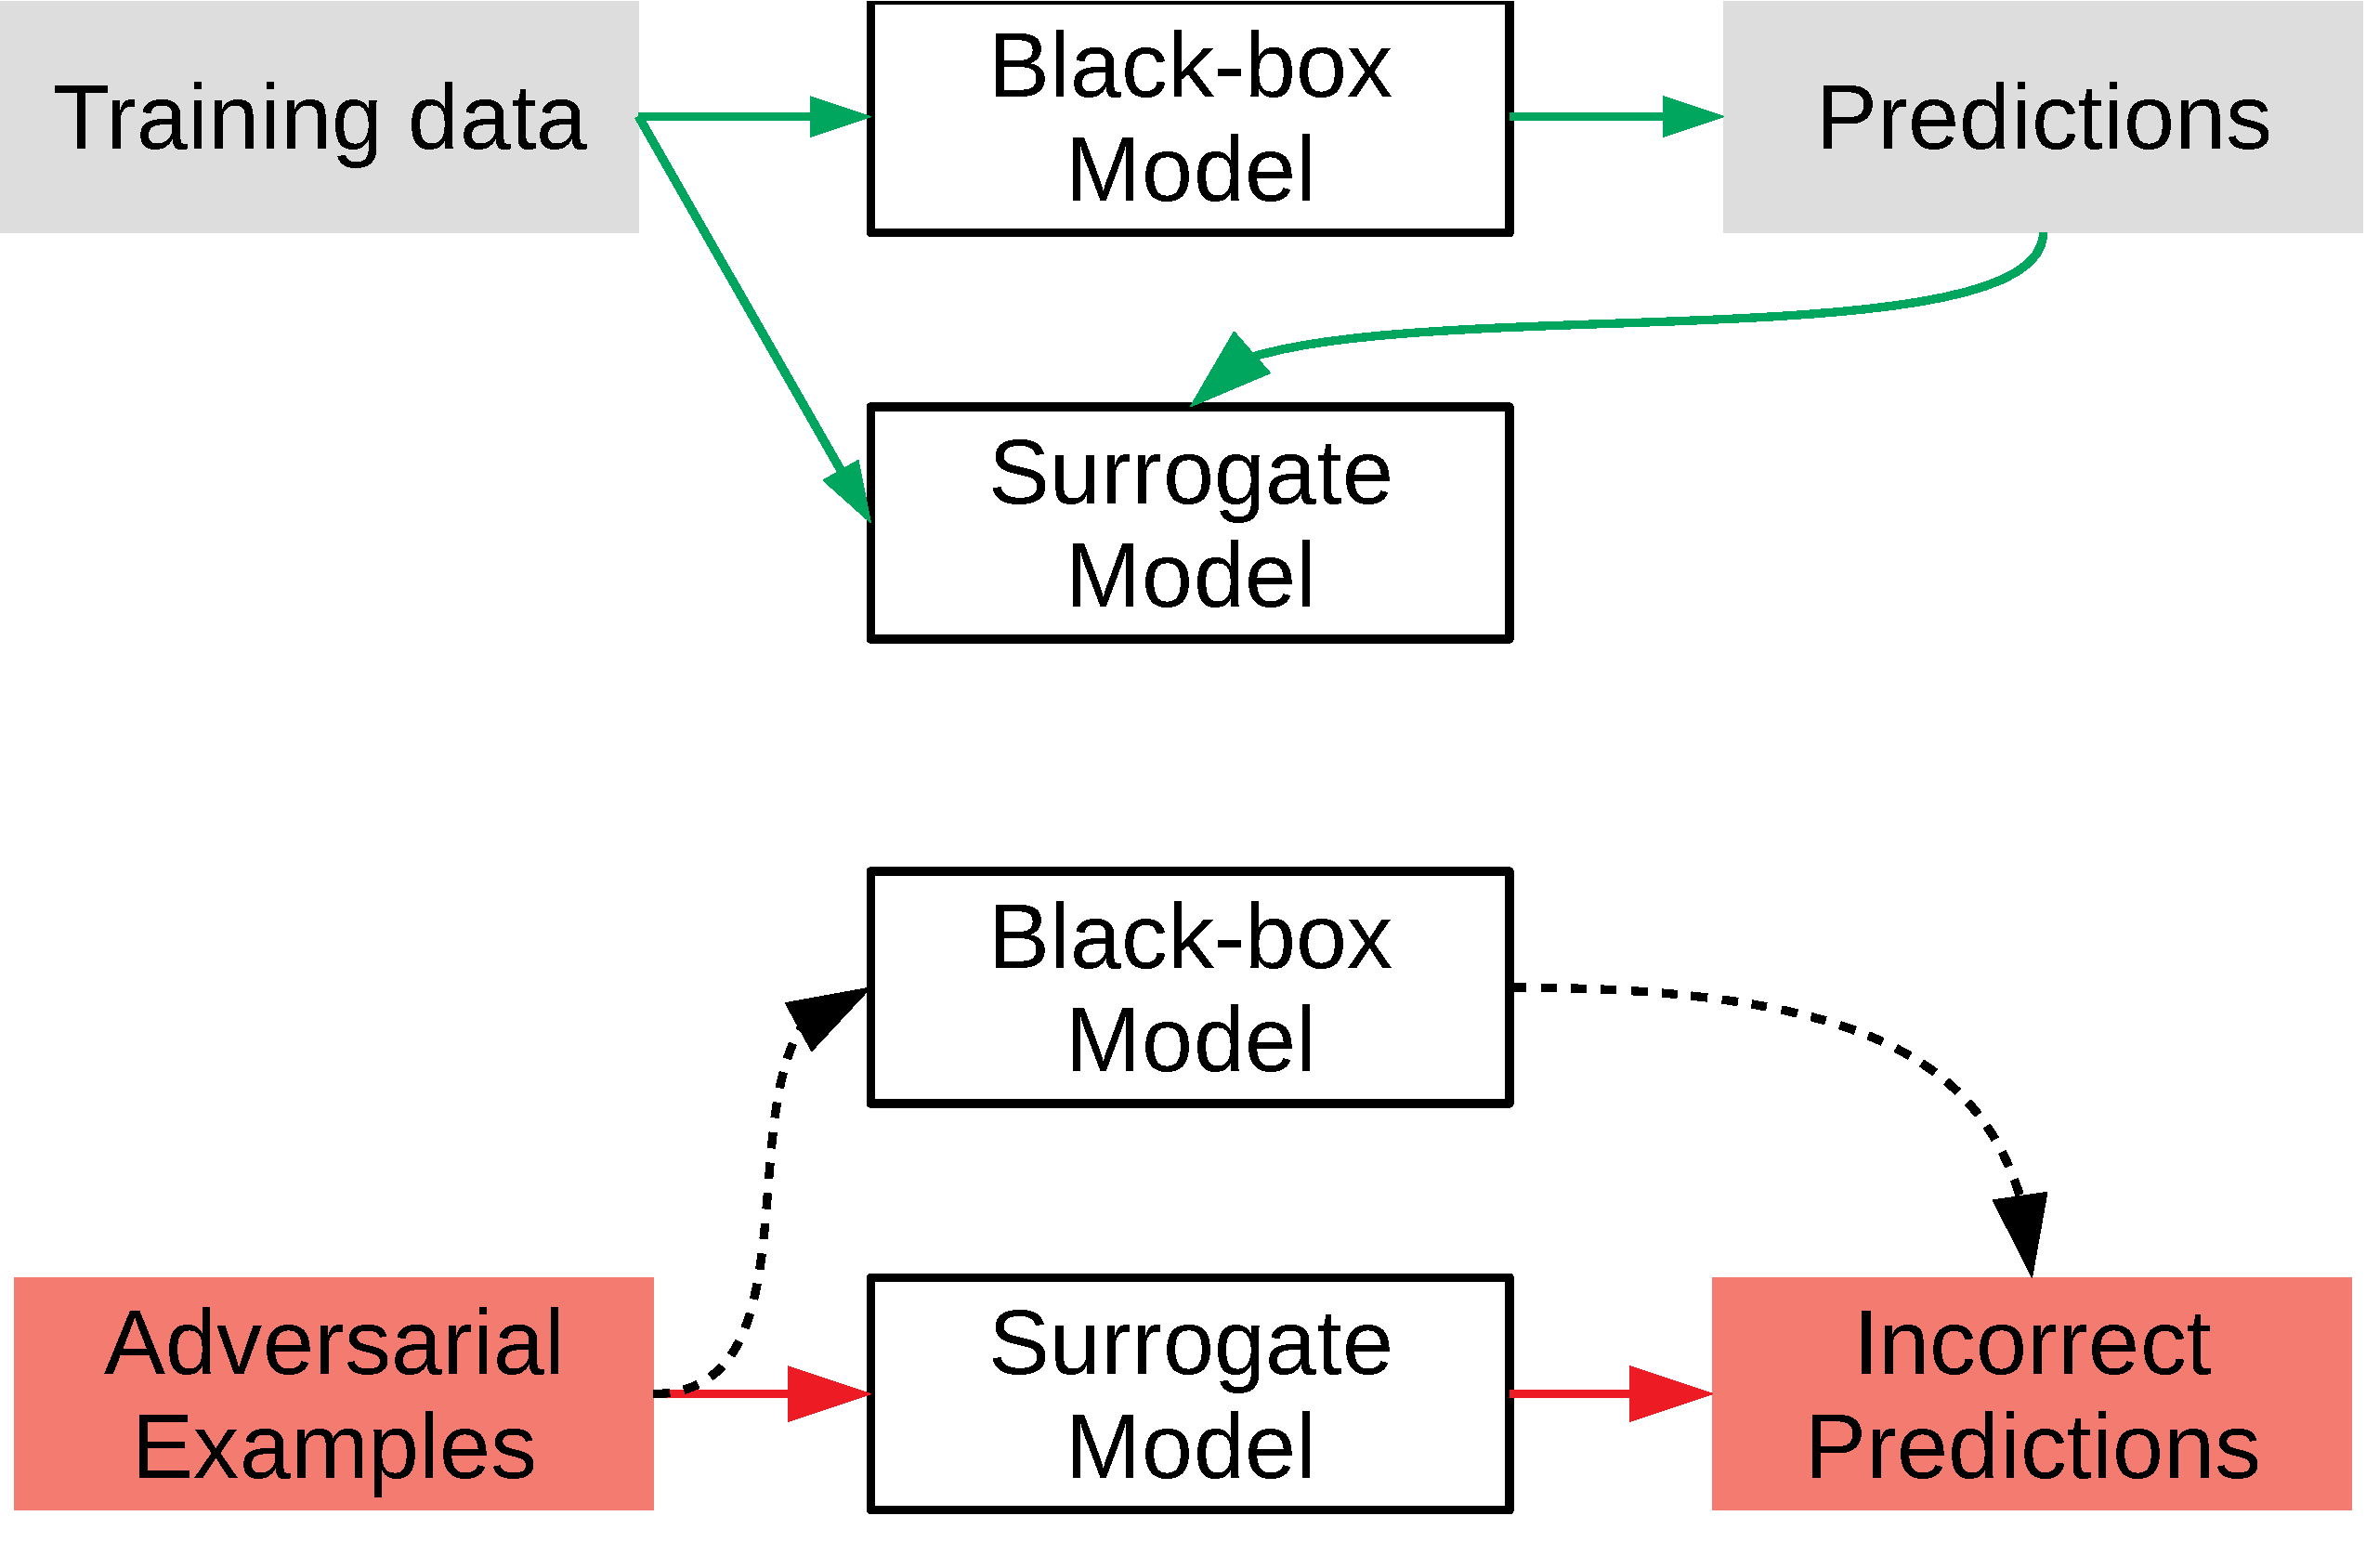
\includegraphics[width=0.8\linewidth]{images/Surrogate model.pdf}
    \caption{Black-box attack can be achieved by training a surrogate model}
    \label{fig:surrogate}
\end{figure}
\end{frame}

%---------------------------------------------------------
\begin{frame}{Why do adversarial examples transfer between models?}
\begin{figure}
    \centering
    \small
    \begin{subfigure}[t]{0.4\linewidth}
        \centering
        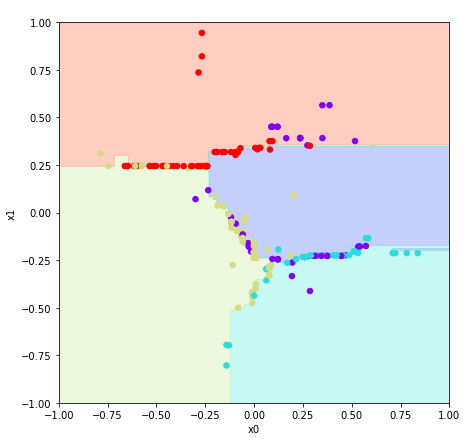
\includegraphics[width=\linewidth]{images/rf.png}
        \caption{Decision boundary of the Random Forest}
    \end{subfigure}
    \hspace{2em}
    \begin{subfigure}[t]{0.4\linewidth}
        \centering
        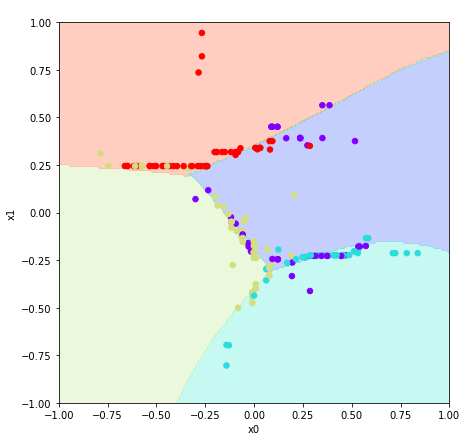
\includegraphics[width=\linewidth]{images/svm.png}
        \caption{Decision boundary of the SVM}
    \end{subfigure}
    \caption{The adversarial examples transferred from RF have \textbf{56.5\%} success rate on SVM}
\end{figure}
\end{frame}

%---------------------------------------------------------
\section{Adversarial Defences}
%---------------------------------------------------------

\begin{frame}{Adversarial defences}
\label{defence}

\begin{itemize}
    \item Preprocessing
    \item Postprocessing
    \item Adversarial retraining
    \item Statistical analysis (\textit{Not applicable to the paradigm below})
\end{itemize}

\begin{figure}
    \centering
    \small
    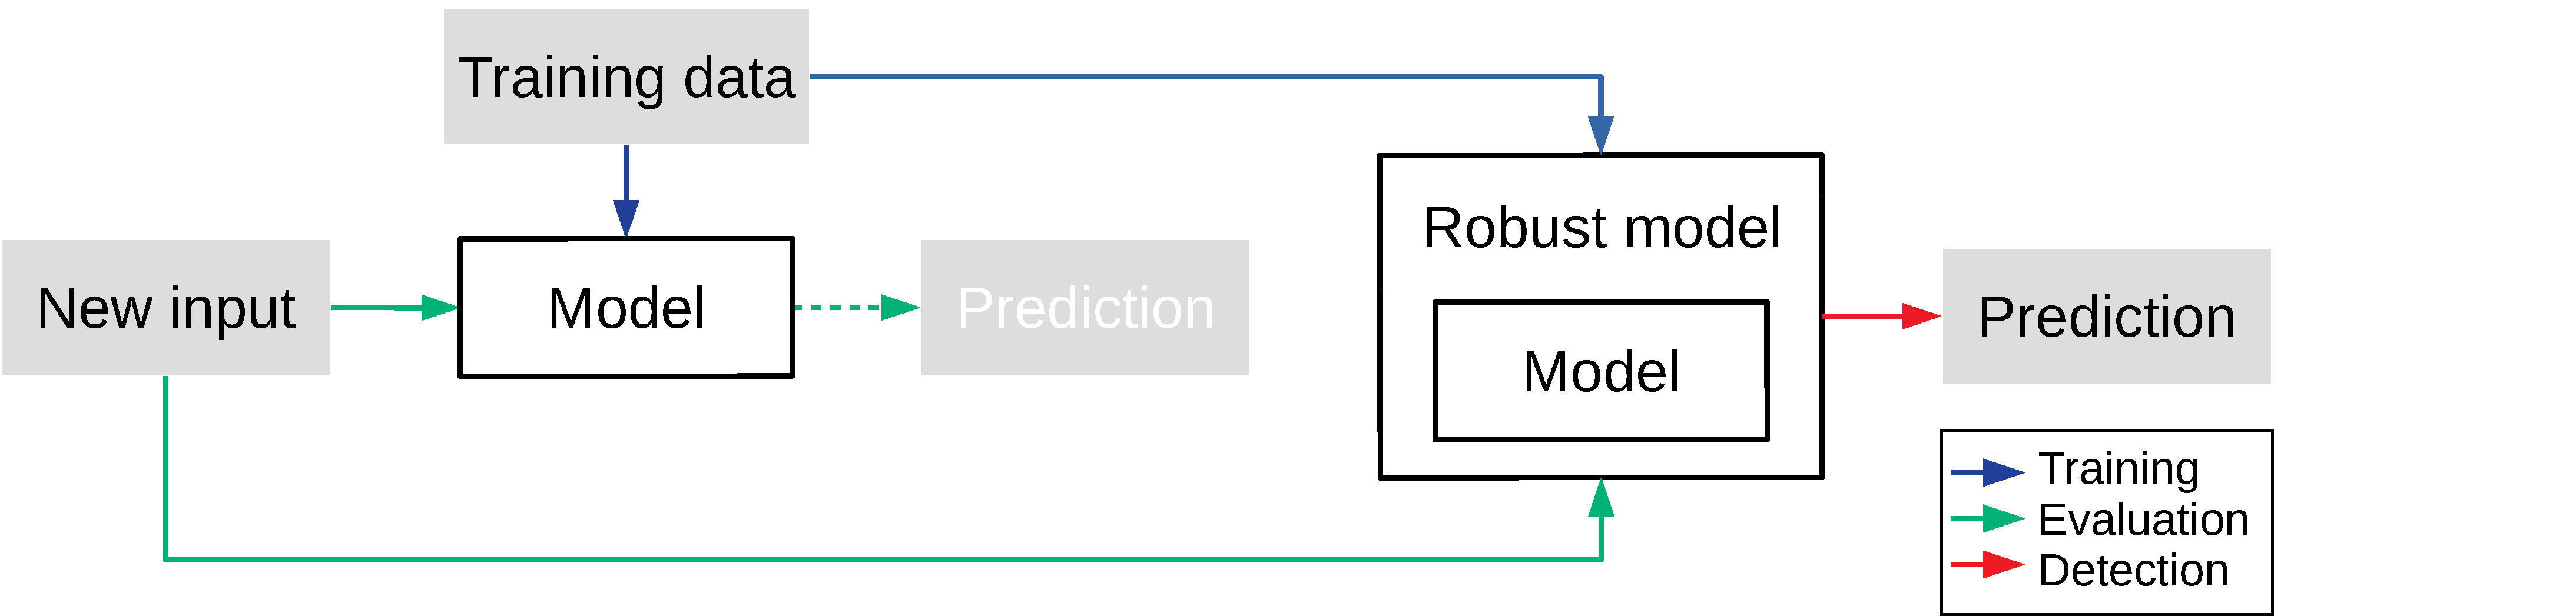
\includegraphics[width=\linewidth]{images/generic-defence.pdf}
    \caption{Generic Adversarial Defence}
    \label{fig:defence}
\end{figure}

\hyperlink{blackbox_defence}{\beamerreturnbutton{Black-box Defence}}
\end{frame}

%---------------------------------------------------------
\begin{frame}{Preprocessing}
\label{preprocessing}

Restore the original inputs from adversarial examples\\
Noise reduction method such as \textbf{PCA}
\begin{examples}
    \begin{figure}
        \centering
        \small
        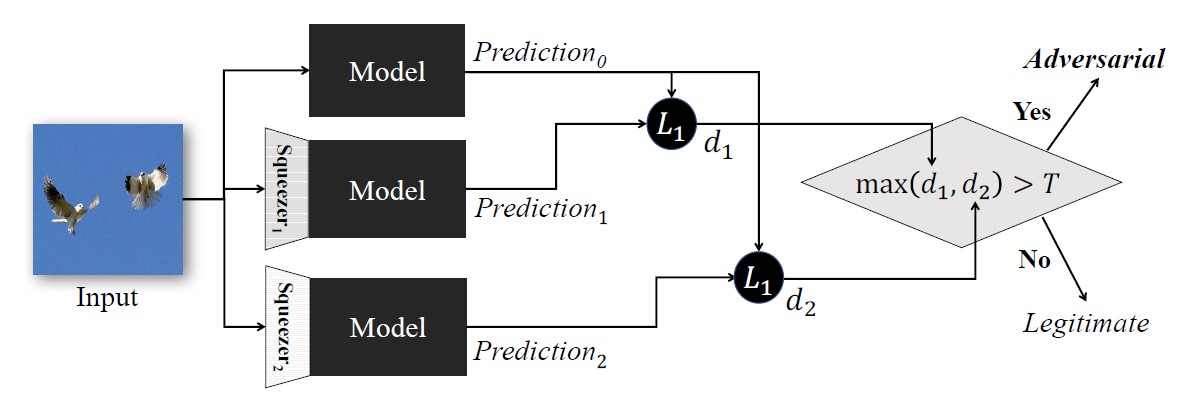
\includegraphics[width=0.8\linewidth]{images/feature_squeezing.jpg}
        \caption{\textbf{Feature Squeezing} trains multiple models with squeezed training set, such as colours depth rescaling, Gaussian blur filter and median filter\footcite{xu2017feature}}
    \end{figure}
\end{examples}

\hyperlink{adv_examples}{\beamergotobutton{Adversarial Examples}}
\end{frame}

%---------------------------------------------------------
\begin{frame}{Postprocessing}

Producing non-reversible outputs
\begin{itemize}
    \item Gradient masking
    \item Defensive distillation
\end{itemize}

\begin{examples}
    \begin{figure}
        \centering
        \small
        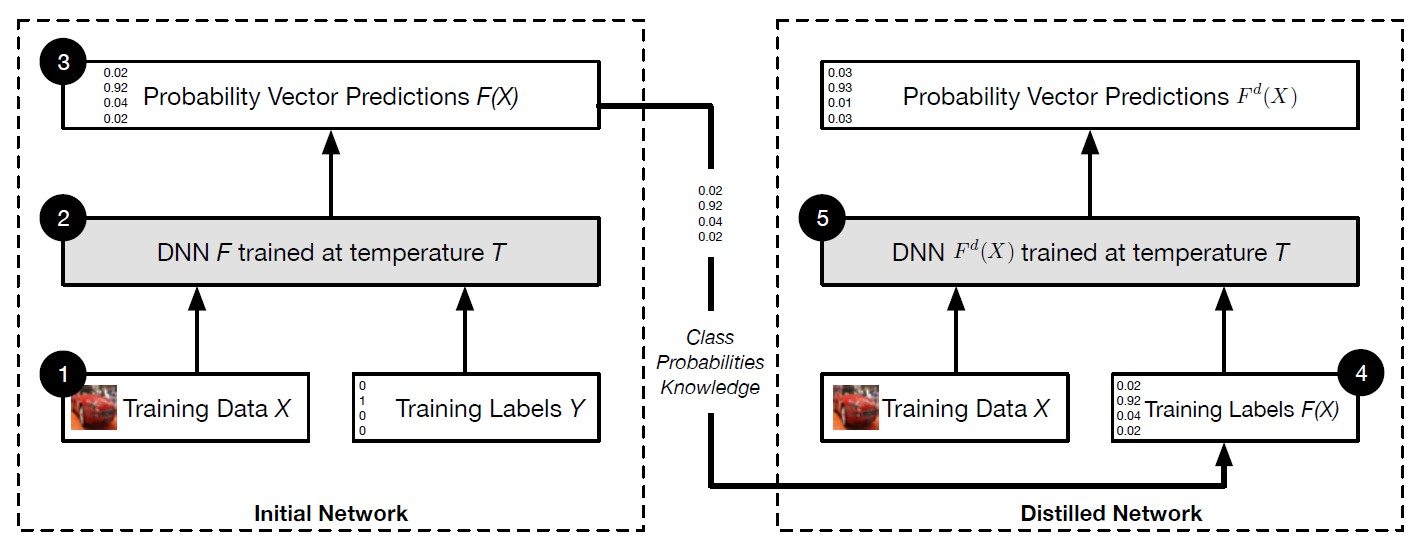
\includegraphics[width=0.8\linewidth]{images/distillation.jpg}
    \end{figure}
    \textbf{Defensive distillation} retrains the data with soft (probability) labels\footcite{papernot2016distillation}.
\end{examples}

\end{frame}

%---------------------------------------------------------
\begin{frame}{Adversarial Retraining}
\label{adv_training}

\begin{itemize}
    \item Injecting a percentage of adversarial examples during training
    \item Weak against unknown attacks
    \item Robust optimisation by Madry {\em et al.}\footcite{madry2017towards}
\end{itemize}

\begin{figure}
    \centering
    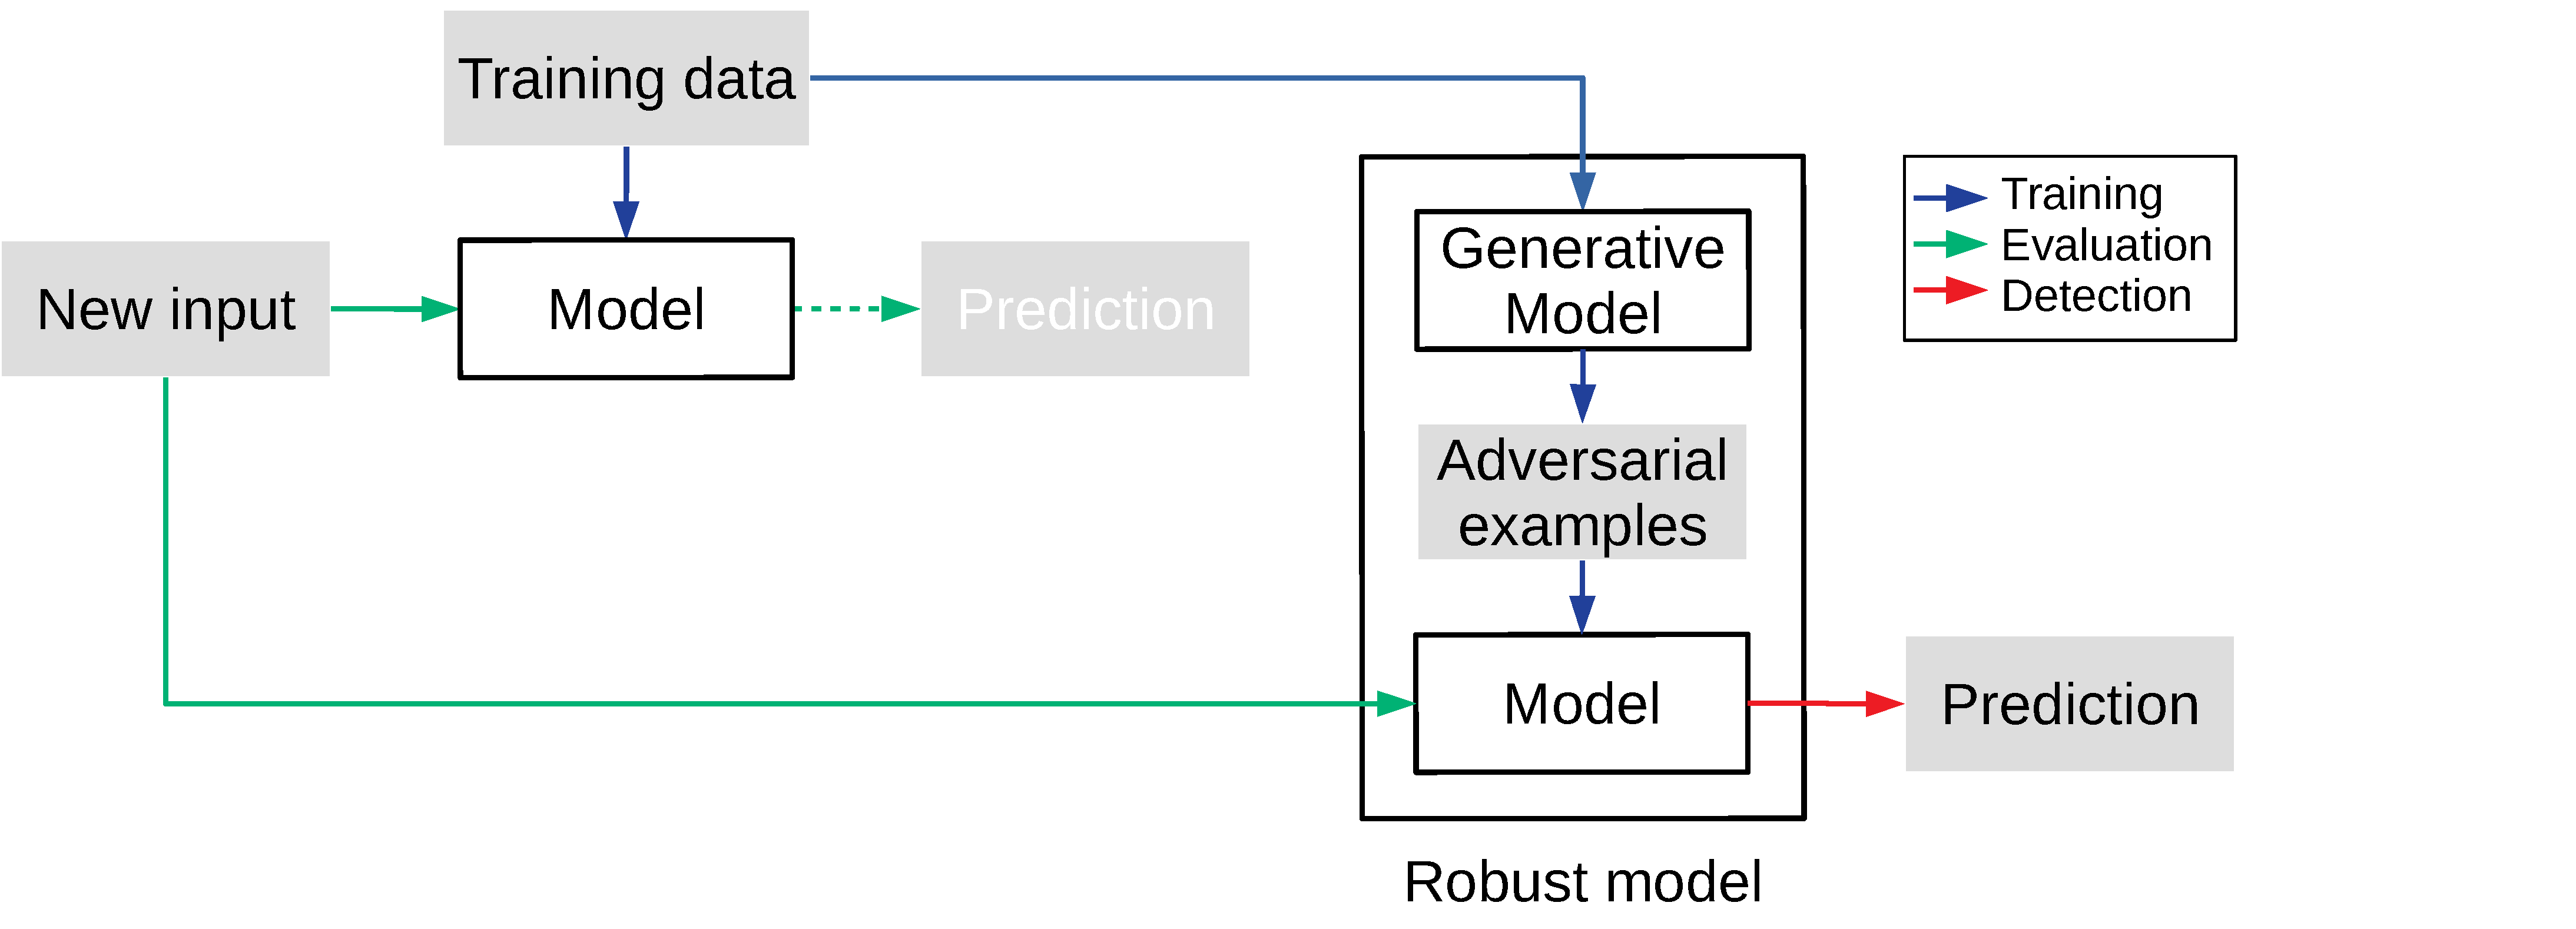
\includegraphics[width=0.8\linewidth]{images/adversarial-training.pdf}
    \caption{Flowchart for Adversarial Retraining}
\end{figure}

\hyperlink{adv_examples}{\beamergotobutton{Adversarial Examples}}
\end{frame}

%---------------------------------------------------------
\begin{frame}{Statistical Analysis}
\label{stats}

Comparing the distribution between adversarial examples and clean training data

\begin{examples}
    \begin{itemize}
        \scriptsize
        \item PCA, t-SNE
    \end{itemize}
\end{examples}

\begin{figure}
    \centering
    \small
    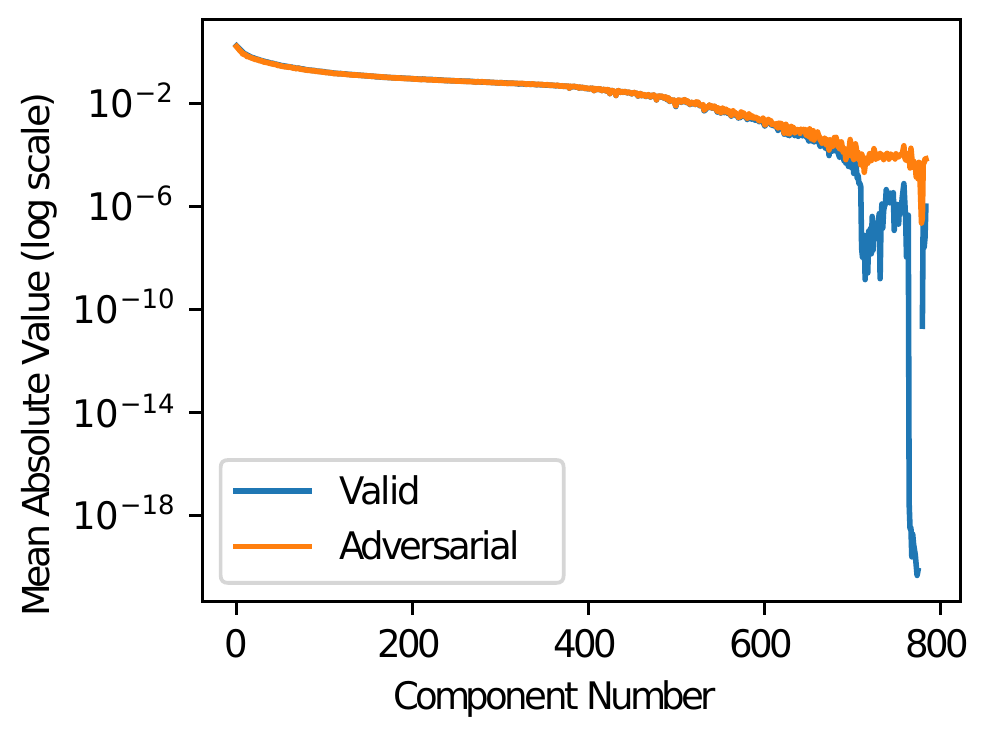
\includegraphics[width=0.3\linewidth]{images/pca.png}
    \caption{The first components have no difference, the difference exists in the tail\footcite{carlini2017adversarial}}
\end{figure}

\hyperlink{adv_examples}{\beamergotobutton{Adversarial Examples}}
\end{frame}

%---------------------------------------------------------
\section{Research Gap in Adversarial Defences}
%---------------------------------------------------------

\begin{frame}{Research Gap in Adversarial Defences}
\textbf{Status Quo}\\
\begin{itemize}
    \item No perfect solution for defending against adversarial examples
    \item No machine learning model is immune to adversarial attacks
\end{itemize}

\vspace{1cm}

\begin{block}{Research Questions?}
    \begin{itemize}
        \item What if the defender has limited access to the model?\\e.g. \textit{Google Cloud AutoML} and \textit{Amazon SageMaker Autopilot}
        \item How can we avoid sacrificing performance on clean inputs?
        \item How can we block adversarial transferability?
    \end{itemize}
\end{block}

\end{frame}

\begin{frame}{Black-box Defence}
\begin{figure}[h!]
    \centering
    \scriptsize
    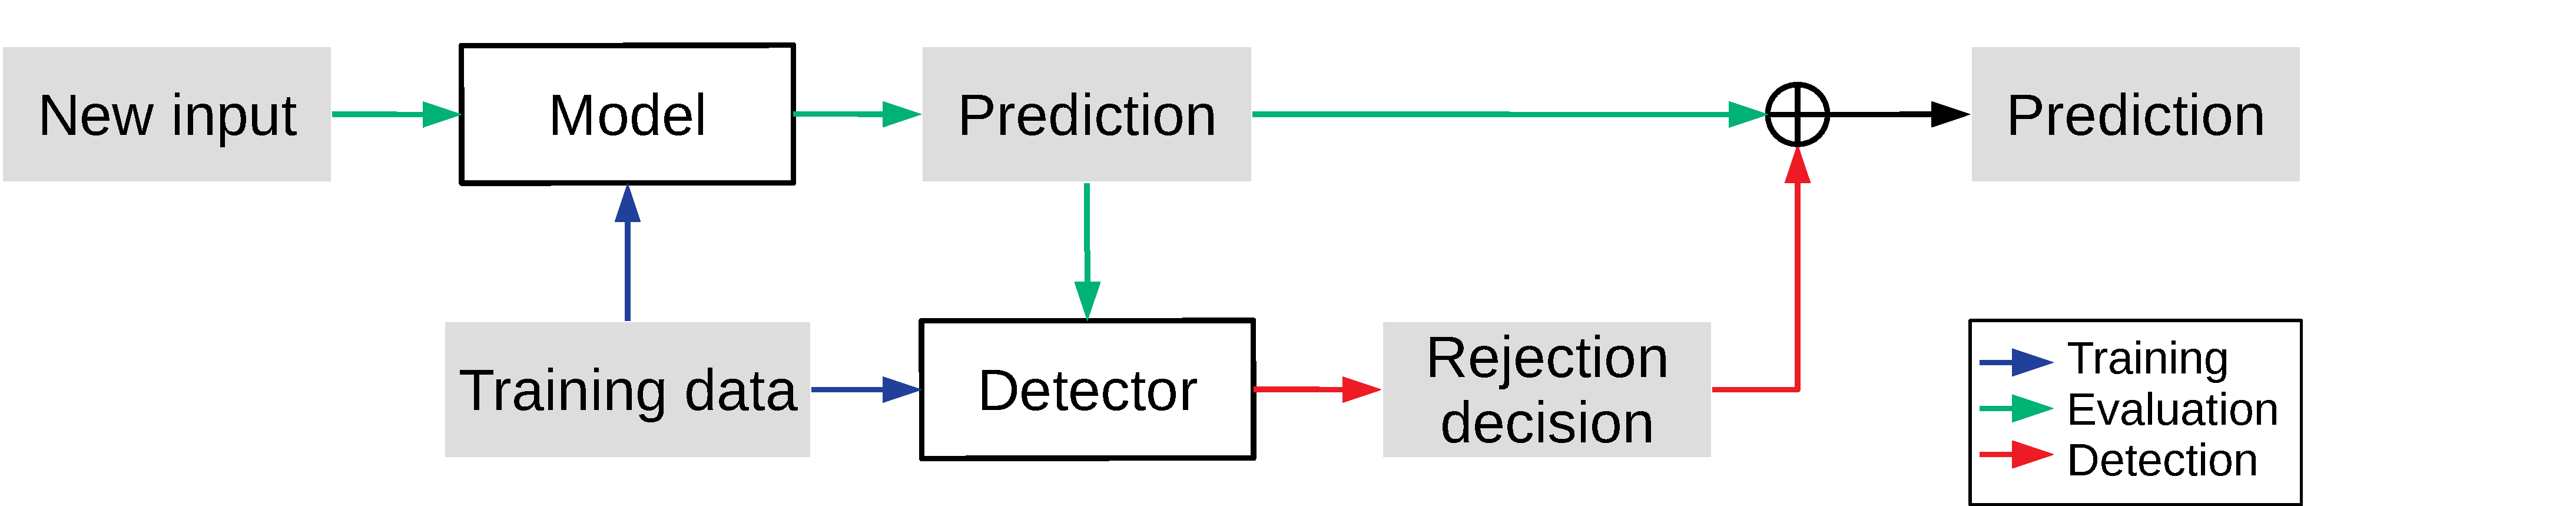
\includegraphics[width=\linewidth]{images/black-box-defence.pdf}
    \caption{Black-box Defence}
\end{figure}

\begin{enumerate}
    \item \textbf{Generic}: The defence should be applicable to a broad variety of data, ML models, and adversarial attacks.
    \item \textbf{Lightweight}: No retraining is required.
    \item \textbf{Robust}: Being able to detect adversarial examples transferred from surrogate models.
\end{enumerate}

\hyperlink{defence}{\beamergotobutton{White-box Defence}}
\end{frame}

%---------------------------------------------------------
\section{Our Black-box Defence: BAARD}
%---------------------------------------------------------
\begin{frame}{Inspired by Applicability Domain (AD) in QSAR modelling}
\label{ad}

\begin{block}{QSAR Modelling}
\textbf{Quantitative Structure–Activity Relationship} (QSAR) models are classification models used in the chemical and biological sciences
\end{block}

\begin{block}{Applicability Domain (AD)}
AD is used to determine the boundaries of inputs for a given model to ensure reliable and accurate predictions in QSAR modelling

\begin{itemize}
    \item AD estimates the adequacy of a model and the confidence in its predictions
    \item AD removes the chemical compounds which are unsuitable for the model
\end{itemize}
\end{block}

Adversarial Examples can ``fool'' the model indicating they are NOT suitable for the model

\hyperlink{decision_boundary}{\beamergotobutton{Decision Boundary}}
\end{frame}

%---------------------------------------------------------
\begin{frame}{Black-box defence: BAARD}
\label{blackbox_defence}

\textbf{B}locking \textbf{A}dversarial examples by testing for \textbf{A}pplicability, \textbf{R}eliability and \textbf{D}ecidability

We adapt the 3-stage approach proposed by Hanser {\em et al.}\footcite{hanser2016applicability}

\begin{figure}[h!]
    \centering
    \scriptsize
    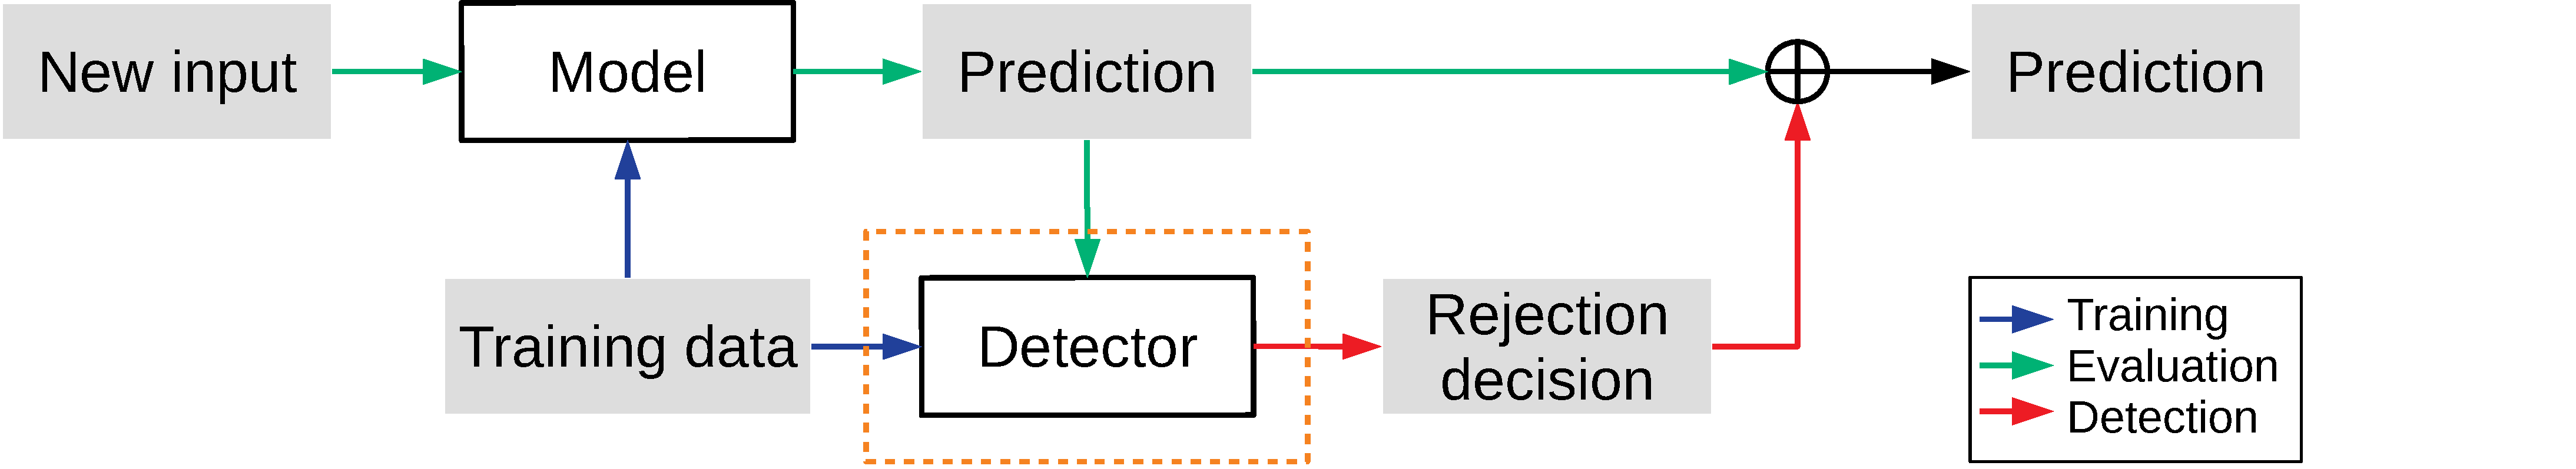
\includegraphics[width=0.7\linewidth]{images/black-box-defence_2.pdf}
    \caption{Black-box Defence}
\end{figure}

\begin{figure}
    \centering
    \scriptsize
    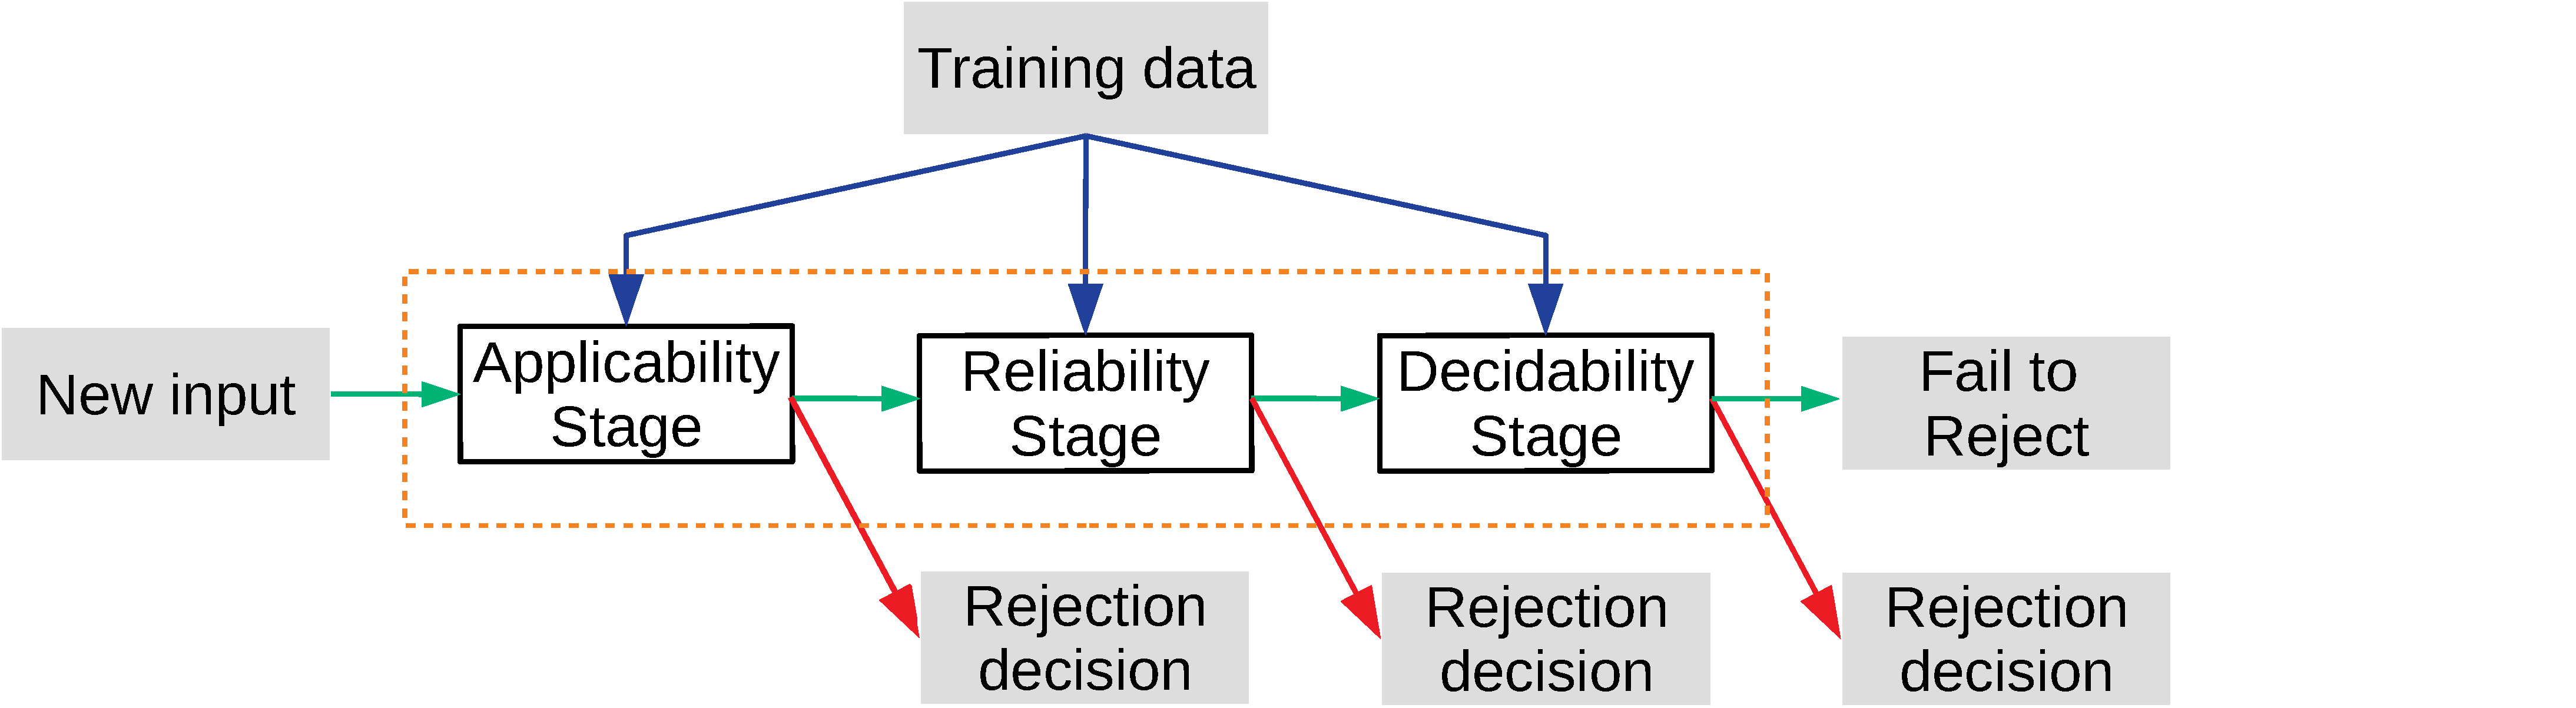
\includegraphics[width=0.7\linewidth]{images/baard_2.pdf}
    \caption{Flowchart of BAARD\footnote{BAARD also uses the predictions from the model. It is omitted to simplify the illustration.}}
\end{figure}
\end{frame}

%---------------------------------------------------------
\begin{frame}{Applicability Stage}
Is the input compliant with the intended use case of the model?
\begin{figure}
    \centering
    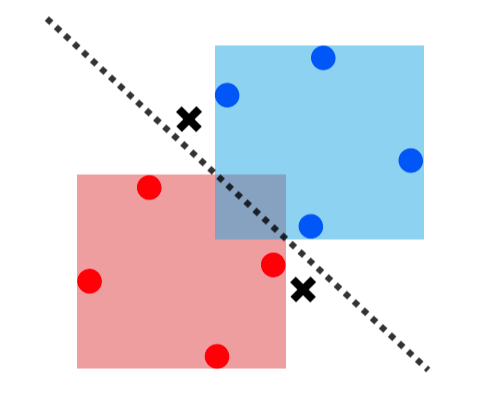
\includegraphics[width=0.35\linewidth]{images/applicability.png}
\end{figure}

\begin{itemize}
    \item Adversarial examples may fall out of the applicable domain of the ML model
    \item Sanity check based on the problem domain (e.g. A house price prediction model receives a new input with -1 bedrooms)
    \item This stage blocks the input if it is not within any one of the \textbf{bounding boxes}
    \item Multiple bounding boxes; One bounding box per class
\end{itemize}

\end{frame}

%---------------------------------------------------------
\begin{frame}{Reliability Stage}
\label{reliability}

Can the model make a reliable prediction?

\begin{figure}
    \centering
    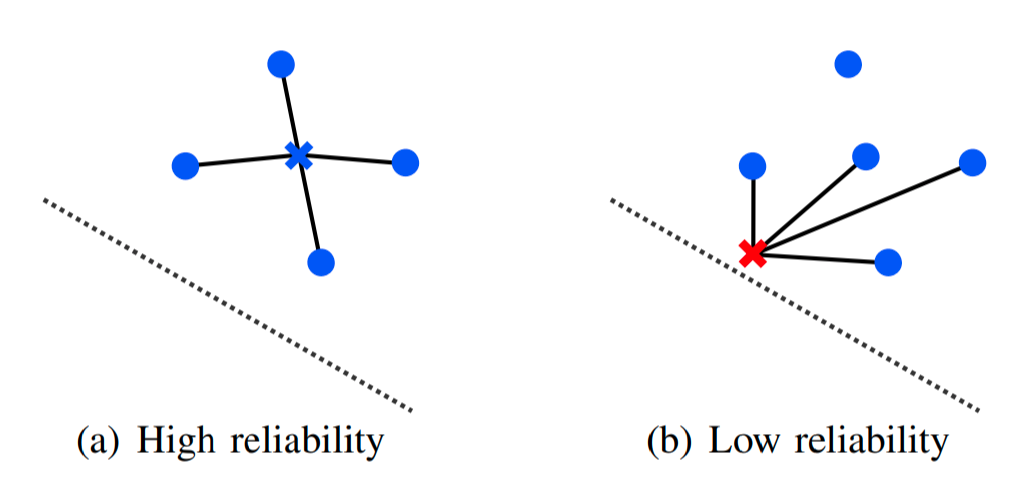
\includegraphics[width=0.6\linewidth]{images/reliability.png}
\end{figure}

\begin{itemize}
    \item Adversarial examples are often close to the decision boundary
    \item Adversarial examples may not in the reliable region in the feature space
    \item This stage is based on the mean \textbf{distance} between the input and its in-class neighbours
    \item Multiple nearest-neighbour models; One model per class
\end{itemize}

\hyperlink{decision_boundary}{\beamergotobutton{Decision Boundary}}
\end{frame}

%---------------------------------------------------------
\begin{frame}{Decidability Stage}
Can the model make a clear decision based on the outcome of a prediction?

\begin{figure}
    \centering
    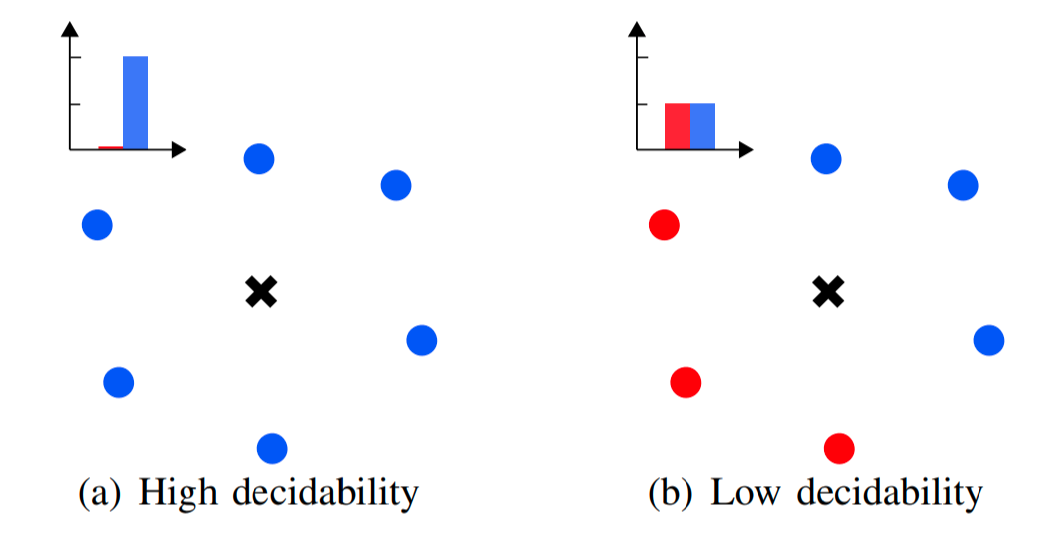
\includegraphics[width=0.6\linewidth]{images/decidability.png}
\end{figure}

\begin{itemize}
    \item Adversarial examples may have less informative label \textbf{distribution} of the neighbours for making decision
    \item This stage is based on the distribution of labels of the nearest neighbours
    \item One nearest-neighbour model; Train on entire training set
\end{itemize}

\end{frame}

%---------------------------------------------------------
\begin{frame}{Results}

\begin{table}[ht!]
    \centering
    \tiny
    \caption{f1 scores}
    \label{tab:f1}
    \begin{tabularx}{\linewidth}{|c|c|*{10}{Y|}}
        \hline
        \multirow{2}{*}{DEFENCE} & \multicolumn{10}{c|}{DATASET} \\ \cline{2-11} 
        & \rotatebox[origin=c]{90}{Iris} & \rotatebox[origin=c]{90}{BankNote} & \rotatebox[origin=c]{90}{WheatSeed} & \rotatebox[origin=c]{90}{HTRU2} & \rotatebox[origin=c]{90}{BreastCancer} & \rotatebox[origin=c]{90}{MNIST} & \rotatebox[origin=c]{90}{CIFAR-Basic} & \rotatebox[origin=c]{90}{CIFAR-ResNet} & \rotatebox[origin=c]{90}{SVHN-Basic} & \rotatebox[origin=c]{90}{SVHN-ResNet} \\ \hline
        AdvTraining & 0.5344 & 0.7372 & 0.6736 & 0.9280 & \textbf{0.8014} & 0.8586 & 0.8662 & \textbf{0.9064} & \textbf{0.8821} & 0.9262 \\
        Destillation & 0.4232 & 0.4678 & 0.6399 & 0.8992 & 0.5538 & 0.6949 & 0.7553 & 0.7236 & 0.7403 & 0.7813 \\
        Squeezing & 0.6767 & 0.6482 & \textbf{0.7498} & 0.9446 & 0.7905 & 0.8375 & \textbf{0.8897} & 0.8247 & 0.8170 & 0.8590 \\
        \textsc{Baard} & \textbf{0.7781} & \textbf{0.9160} & 0.7377 & \textbf{0.9455} & 0.5367 & \textbf{0.8964} & 0.8338 & 0.8622 & 0.8722 & \textbf{0.9385} \\ \hline
    \end{tabularx}
\end{table}

Only BAARD does not retrain the ML model.

\end{frame}

%---------------------------------------------------------
\begin{frame}{Results on neural network models}

\begin{figure}
    \centering
    \includesvg[width=\linewidth]{images/box_result_mnist}
    \caption{Number of blocked adversarial examples on MNIST}
\end{figure}

\end{frame}

%---------------------------------------------------------
\section{The Big Picture}
%---------------------------------------------------------

\begin{frame}{The Big Picture}
Evaluation Matrix

\begin{itemize}
    \item Considering the dataset and the model as a pair
    \item Establishing a scoring system which can be used to evaluate the robustness of the data given a ML model
    \item To better understand how the data and the model work together
\end{itemize}

\begin{figure}[h!]
    \centering
    \scriptsize
    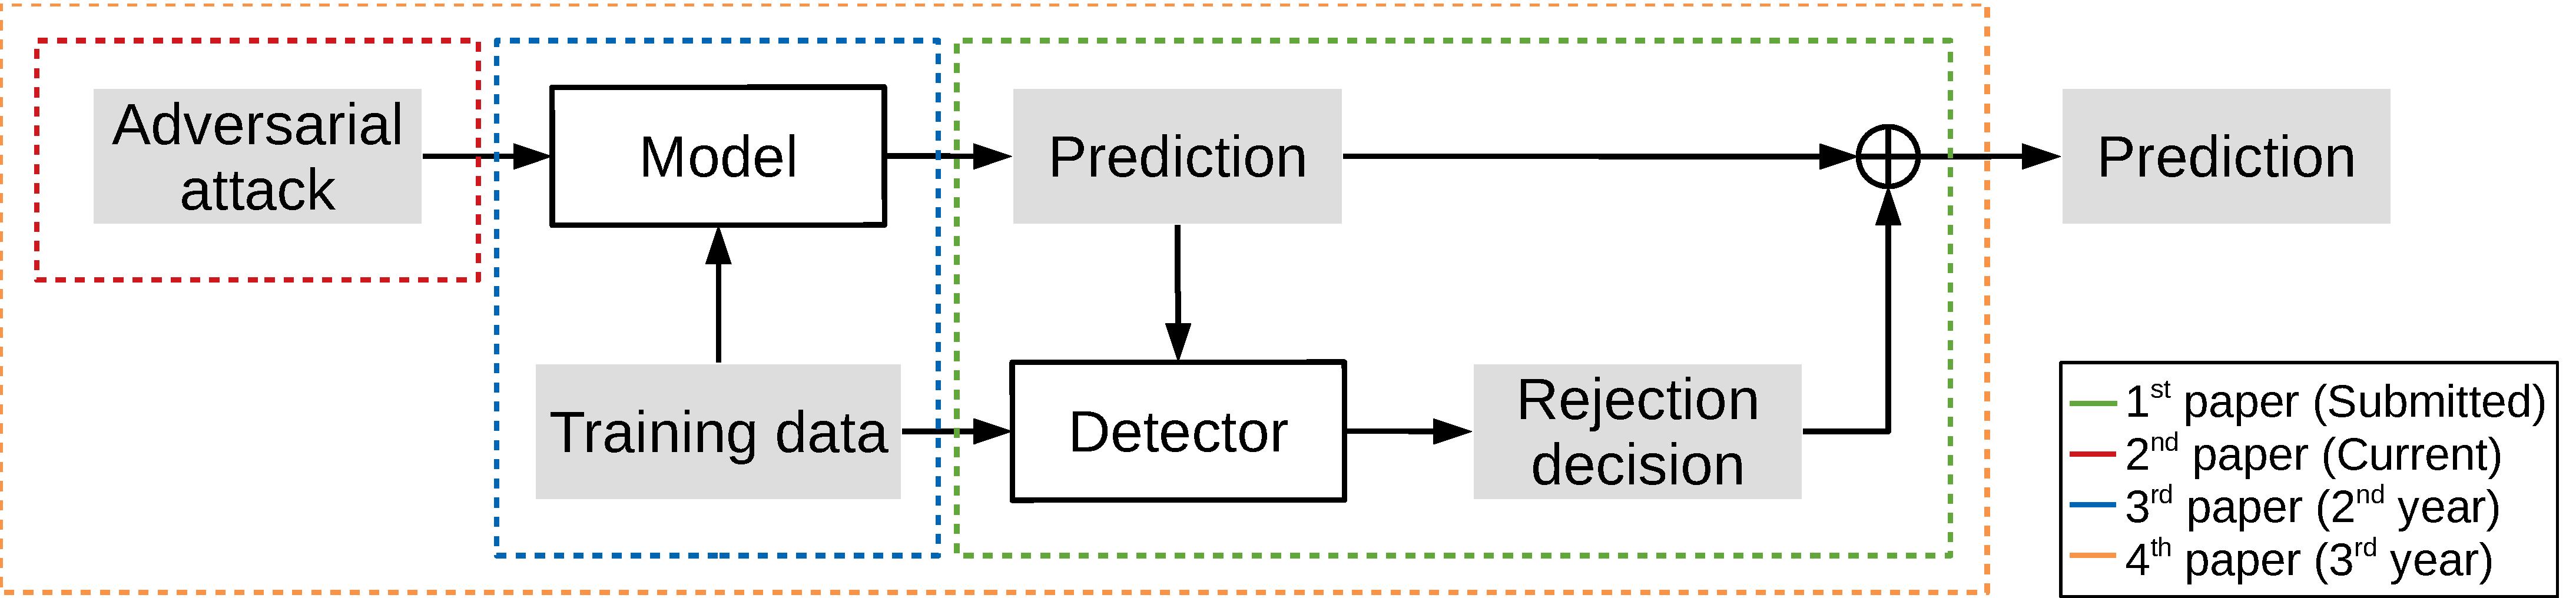
\includegraphics[width=\linewidth]{images/paper-timeline-diagram.pdf}
    \caption{Plan for the future work}
    \label{fig:timeline-boxes}
\end{figure}

\end{frame}

%---------------------------------------------------------
\section{Timeline}
%---------------------------------------------------------

\begin{frame}{First Year - Preliminary Research and Prototype Development}

\begin{table}
\centering
\scriptsize
\setlength\extrarowheight{6pt}
\arrayrulecolor{lightgray}
\setlength\arrayrulewidth{1pt}
\begin{tabular}{@{\,}r <{\hskip 2pt} !{\timeline} >{\raggedright\arraybackslash}p{0.8\textwidth}}
Oct 19          & Started PhD\\
Oct 19 - Dec 20 & Background study\\
Jan 20          & Proof of concept that Applicability Domain can be applied to defend adversarial attacks\\
Feb 20 - Apr 20 & Implemented a novel adversarial defence - BAARD and conducted extensive experiments\\
May 20 - Jul 20 & Wrote and submitted a full paper to ICDM 2020 (\nth{1} paper)\\
Jul 20 & 3MT presentation on defending adversarial attacks using BAARD\\
Aug 20          & Composing a new algorithm for white-box attack on Random Forest models\\
Sep 20          & Developed the concept of black-box defence based on BAARD\newline Reworked the paper and submitted to AAAI 2021 (resubmitted \nth{1} paper)\\
Oct 20          & Preparing for the Provisional Year Review\\
\end{tabular}
\end{table}

\end{frame}

%---------------------------------------------------------
\begin{frame}{After Provisional Year}

\begin{table}
\centering
\scriptsize
\setlength\extrarowheight{6pt}
\arrayrulecolor{lightgray}
\setlength\arrayrulewidth{1pt}
\begin{tabular}{@{\,}r <{\hskip 2pt} !{\timeline} >{\raggedright\arraybackslash}p{0.8\textwidth}}
\textbf{Second Year} & \textbf{Developing and Evaluating the Evaluation Matrix}\\
Oct 20 - Dec 20 & Continue working on white-box attacks and defences\\
Jan 21 - Feb 21 & Writing a paper for white-box attacks and defences (\nth{2} paper)\\
Mar 21 - Jun 21 & Quantifying the robustness of adversarial defences;\newline
Constructing an evaluation matrix to estimate the robustness of a dataset based on these characteristics\\
Jul 21 - Oct 21 & Conducting experiments for evaluating the adversarial evaluation matrix;\newline
Writing a paper for the adversarial evaluation matrix (\nth{3} paper)\\
\hline
\textbf{Third Year} & \textbf{Analysing Limitations and Preparing Thesis}\\
Nov 21 - Jan 21 & Applying the existing research output to a wider range of data\\
Feb 21 - Apr 21 & Analysing the limitation of current approaches;\newline
Writing a paper for analysing the expandability and limitation of the adversarial evaluation matrix (\nth{4} paper)\\
May 21 - Oct 21 & Writing the PhD thesis and preparing the PhD defence\\
Oct 21          & Submit the thesis\\
\end{tabular}
\end{table}

\end{frame}

\end{document}
